\documentclass[review]{elsarticle}

\usepackage{lineno,hyperref}
\usepackage{amsmath}
\modulolinenumbers[5]
\usepackage{graphicx}
\usepackage{caption}
\usepackage{subcaption}
\usepackage{tikz}

\journal{Coastal Engineering}

%%%%%%%%%%%%%%%%%%%%%%%
%% Elsevier bibliography styles
%%%%%%%%%%%%%%%%%%%%%%%
%% To change the style, put a % in front of the second line of the current style and
%% remove the % from the second line of the style you would like to use.--00
%%%%%%%%%%%%%%%%%%%%%%%

%% Numbered
%\bibliographystyle{model1-num-names}

%% Numbered without titles--
%\bibliographystyle{model1a-num-names}

%% Harvard
%\bibliographystyle{model2-names.bst}\biboptions{authoryear}

%% Vancouver numbered
%\usepackage{numcompress}\bibliographystyle{model3-num-names}

%% Vancouver name/year
%\usepackage{numcompress}\bibliographystyle{model4-names}\biboptions{authoryear}

%% APA style
%\bibliographystyle{model5-names}\biboptions{authoryear}

%% AMA style
%\usepackage{numcompress}\bibliographystyle{model6-num-names}

%% `Elsevier LaTeX' style
\bibliographystyle{elsarticle-num}
%%%%%%%%%%%%%%%%%%%%%%%

\begin{document}

\begin{frontmatter}

\title{Dispersive modeling of breaking waves  on a slope}

%% Group authors per affiliation:
\author[1]{Jihwan Kim}
\author[1]{Geir K. Pedersen}
\author[1,2]{Finn L{\o}vholt}
\author[3]{Randall J. LeVeque}

\address[1]{University of Oslo, Department of Mathematics, 
Oslo, Norway}
\address[2]{Norwegian Geotechnical Institute,
Oslo, Norway}
\address[3]{University of Washington, Department of Applied Mathematics, Seattle, USA}

\begin{abstract}

\end{abstract}

\begin{keyword}

\end{keyword}

\end{frontmatter}

\linenumbers

\section{Introduction}

Depth-averaged models are widely used 
in the study of the tsunami propagation,
and the {\em nonlinear shallow water equations}
are a robust model for its efficiency and accuracy.
The shallow water equations have been used and validated
in the study of destructive tsunami events 
such as the 2004 Indian Ocena tsunami and the 2011 Tohoku tsunami.
However, the details of the waves have not been accurately captured
because the dispersion of waves is not included 
in the shallow water equations.   
The dispersion becomes important in several cases.
When surface waves travel a long distance 
with respect to the wavelength, for example,
the dispersion of waves develops. 
As another case, the waves generated by the submarine landslides
have relatively short wavelength compared to 
the waves generated by the earthquakes,
and the dispersion should be considered for accuracy. 

The {\em Boussinesq-type equations} are 
a class of depth-averaged models
which can handle short waves better than the shallow water equations.
With additional dispersion terms, 
the Boussinesq-type equations can 
address the dispersive motion of wave revolution. 
One of the limitations of the Boussinesq-type equations
arises when a wave breaks near the shoreline. 
Without appropriate modifications, 
the numerical results show that the wave height 
continues to increase and may result in numerical instabilities. 
For this reason, several thresholds have been 
suggested to determine the wave break. 
As the wave break is detected, the governing equations
are switched to the shallow water equations.


\section{Model Description}

The shallow water equations\marginpar{\footnotesize Geir: 
This is too much of a basic introduction. However, let's write the 
introduction section before we change it?}
are a system of hyperbolic partial differential equations
which can be derived from 
the Navier-Stokes' equations
assuming that the vertical velocity is negligible. This leads 
to a hydrostatic pressure and a uniform horizontal speed horizontal 
throughout the depth. 
If waves have long wavelength  
with respect to the depth of water,
the shallow water equations is
a robust and efficient physical model. 
If waves are shorter,
alternative wave models may be preferred 
which can handle dispersive waves. 
The Boussinesq-type equations
is a class of the depth-averaged model 
that can treat shorter waves more accurately
than the shallow water equations. 
The Boussinesq-type wave models have been derived by retaining 
$\mathcal{O}(\epsilon)$ and $\mathcal{O}(\mu)$ terms, 
where $\epsilon$ and $\mu$ 
denote the ratio of wave amplitude to depth
and the ratio of depth to wavelength respectively. 
Various models have been suggested.  
The papers of Peregrine (1967) \citep{peregrine1967long},
Madsen and S{\o}rensen (1992) \citep{madsen1992new}, Nwogu (1993) \citep{nwogu1993alternative}, Lynett et al. (2002) \cite{lynett2002modeling},
and Wei and Kirby (1995) \citep{wei1995time}
are representative examples. 

In this work, a new numerical tool, 
called {\em WaveClaw}, is introduced. 
It is an extension of \textsc{Geoclaw} \citep{clawpack}.
That solves 
the Boussinesq-type equations derived by
Sch{\"a}ffer et al. (1993) \citep{schaffer1993boussinesq}.
The \textsc{WaveClaw}
is a hybrid of the finite volume and finite difference solvers
with the operation splitting technique.
The \textsc{Geoclaw} software is 
a part of \textsc{Clawpack} \citep{clawpack}
by LeVeque (1997) \cite{leveque1997wave}, George (2008) \citep{george2008augmented} and Berger et al. (2011) \citep{BergerGeorgeLeVequeMandli11}
which solves the nonlinear shallow water equations.
%with properties such as high-resolution, total variation diminishing (TVD) and adaptive mesh refinements (AMR).
% The wave propagation algorithms by LeVeque (1997) \cite{leveque1997wave} is implemented, and the steady state is preserved. 

\subsection{\textsc{WaveClaw}}

\subsubsection{Boussinesq-type equations}

Sch{\"a}ffer et al. (1993) \citep{schaffer1993boussinesq} derived 
Boussinesq-type equations
with an addition of a Pad{\'e} approximation 
of the linear dispersion relation.
The  equations read 
\begin{flalign}
& H_t + (Hu)_x  = 0, \label{eq:madsen_cons_mass} & \\ 
& (1-D)\big\lbrack(Hu)_t\big\rbrack + \left( Hu^2 + \frac{g}{2}H^2 \right)_x - gHh_x -Bgh^2\left(h\eta_x\right)_{xx} =0, & \label{eq:madsen_momx}
\end{flalign}
where the operator, $D$, is defined as
\begin{flalign}
 D (w) &= \left(B+\frac{1}{2} \right)h^2 w_{xx} -\frac{1}{6} h^3 \left(\frac{w}{h}\right)_{xx}, & \label{eq:madsen_new_op}
\end{flalign}
for any $w(x,t)$.
In the above equations $H(x,t)$ and $u(x,t)$ are the total flow depth and velocity of the water, respectively, 
$h(x)$ is the still water depth, $\eta(x,t)$ is the surface elevation,
and thus $H(x,t)=h(x)+\eta(x,t)$. 
Moreover, $g$ is the acceleration of gravity, 
and $B$ is a dispersion parameter. 
Madsen and S{\o}rensen (1992) \cite{madsen1992new} 
has chosen the parameter $B=1/15$ 
from a Pad{\'e}
expansion of the linear dispersion analysis.

When $B=0$, this set of the Boussinesq-type equations
approximately reduces to that of Peregrine (1967) \citep{peregrine1967long}
as the linear dispersion relations are identical. 
However, unlike Peregrine's momentum equation the hydrostatic parts of  (\ref{eq:madsen_momx}) are written in a conservative form.
This difference will be observed in the numerical procedure and is
further elaborated in \ref{append:a}.

The \textsc{WaveClaw} software
solves the Boussinesq-type equations (\ref{eq:madsen_cons_mass}) and (\ref{eq:madsen_momx}) numerically
with a hybrid of the finite volume and finite difference methods. 
There have been several studies on this type of hybrid schemes.
For example, see Tisser et al. (2011) \cite{tissier2011serre}, 
Shi et al. (2012) \cite{shi2012high} 
and Dutykh et al. (2013) \cite{dutykh2013finite}.


To facilitate a fractional step method, as outlined below, we move the hydrostatic terms of (\ref{eq:madsen_momx}) inside the $(1-D)$ 
operator, while balancing with extra terms in the $\Psi$, to obtain
\begin{flalign}
& (1-D)\big\lbrack (Hu)_t + \left(Hu^2 + \frac{g}{2}H^2 \right)_x - gHh_x\big\rbrack = -\Psi(x,t), & \label{eq:hybrid_src}
\end{flalign}
where
\begin{flalign}
\Psi(x,t)= & \left(B+\frac{1}{2} \right) h^2 \left( (Hu^2)_{x} + g H \eta_x \right)_{xx} \nonumber\\
& -\frac{1}{6}h^3 \left( \frac{ (Hu^2)_x +gH\eta_x }{h} \right)_{xx}
-Bgh^2\left(h\eta_x\right)_{xx}. &
\label{eq:madsen_new_disp_x}
\end{flalign}

\subsubsection{Numerical scheme}

The equations (\ref{eq:madsen_cons_mass}) and (\ref{eq:hybrid_src}) are 
written in a form that is conserves momentum to leading order in $\mu$, but with the $\Psi$
term as a pseudo source.
Such equations may be solved  
by a {\em fractional step method} as described in  
 LeVeque (2002) \cite{leveque2002finite},
for instance. 
First, it is observed that (\ref{eq:hybrid_src}) may be formally
rewritten as 
\begin{flalign}
& (Hu)_t =- \left\lbrace\left(Hu^2 + \frac{g}{2}H^2 \right)_x - gHh_x\right\rbrace -(1-D)^{-1}\Psi(x,t), & \label{eq:hybrid_inv}
\end{flalign}
At the first stage of the hybrid scheme, we integrate $Hu$ over a time step
taking into account all hydrostatice terms on the right hand side, namely 
those within the braces and dropping the source terms involving $\Psi$. 
When this is combined with the continuity equation
  (\ref{eq:madsen_cons_mass}) this simply corresponds to advancing NLSW equations one time step forward. To this end we employ ...... from GEOCLAW.\marginpar{\small add a descriptio of the NLSW procedure}
In the second stage, we retain the new $H$ value, but integrate $Hu$ (essentially being the momentum density) further 
from the first stage by solving
\begin{flalign}
& \left(1-D \right)\big\lbrack (Hu)_t\big\rbrack = -\Psi . & \label{eq:hybrid_mom_fdm}
\end{flalign}
Since the differential operator $D$ contains spatial derivatives,
a systems of difference equations must then be solved. 

The spatial and time discretization should be carefully chosen 
for the stability of the second stage. 
In our numerical scheme, the second order centered scheme
is used for the spatial discretization, 
and a four stage Runge-Kutta method is used for the time integration.
The von Neumann stability analysis of this numerical scheme 
is outlined in \ref{append:stab}.

Suppose the spatial domain is divided into $n$ grid cells with 
the spatial grid size $\Delta x$.
Arrays of nodal values for flow depth and $Hu$, respectively, are
defined as
\begin{flalign*}
\textbf{H} & =
(H_1,H_2, \dots , H_n)^T, & \\
\textbf{M} & =
(H_1u_1,H_2u_2, \dots , H_nu_n)^T. &
\end{flalign*}

With time increment $\Delta t$ the fourth order Runge-Kutta scheme
can be written as follows,
\begin{flalign*}
\textbf{M}^1 = \textbf{M}, \quad 
\textbf{M}^2 = \textbf{M} + \frac{\Delta t}{2}\textbf{S}^1, \quad
\textbf{M}^3 = \textbf{M} + \frac{\Delta t}{2}\textbf{S}^2, \quad
\textbf{M}^4 = \textbf{M} + \Delta t \textbf{S}^3,
\end{flalign*}
where $\textbf{M}^k$ are intermediate value arrays\marginpar{How are values for $H$ obtained in the steps; linear interpolation ?} 
and $\textbf{S}^k$ are
correpondingly arrays for the time derivatives of $Hu$, obtained by
solving 
\begin{flalign}
(I-\bar{D})\textbf{S}^k & 
= -\bar{\Psi}(\textbf{H},\textbf{M}^k), \quad \textrm{for~} k=1,\dots,4. &
\label{eq:rk4_1}
\end{flalign}
Here $\bar{\Psi}$ and $\bar{D}$ represent centered spatial discretizations for the term $\Psi$ and the operator $D$, respectively. These
are given explitly below.
Finally the value of $\textbf{M}$ at the new time level is
obtained by
\begin{flalign*}
\textbf{M}^+ & = \textbf{M} + \frac{\Delta t}{6} \left[
\textbf{S}^1+2\textbf{S}^2+2\textbf{S}^3+\textbf{S}^4
\right]. &
\end{flalign*}

In (\ref{eq:rk4_1}), 
$\bar{D}$ is a tri-diagonal $n\times n$ matrix with elements 
\begin{flalign*}
 \bar{D}_{i,i-1} = & \frac{1}{\Delta x^2} \left[
 \left(B + \frac{1}{2} \right) h_i^2 
-\frac{1}{6} \frac{h_i^3}{h_{i-1}} \right],  & \\
 \bar{D}_{i,i} = & \frac{1}{\Delta x^2}
 \left(-2B - \frac{2}{3} \right) h_i^2 ,  & \\
 \bar{D}_{i,i+1} = & \frac{1}{\Delta x^2} \left[
 \left(B + \frac{1}{2} \right) h_i^2 
-\frac{1}{6} \frac{h_i^3}{h_{i+1}} \right].  & 
\end{flalign*}
Correspondingly, the $i$-th element of $\bar{\Psi(\textbf{H},\textbf{q})}$ is 
\begin{flalign*}
\bar{\Psi}_i 
&=  \left(B+\frac{1}{2} \right) \frac{h_i^2}{2\Delta x^3} 
\Bigg[
\left(\frac{M_{i+2}^2}{H_{i+2}} -2\frac{M_{i+1}^2}{H_{i+1}} 
+2\frac{M_{i-1}^2}{H_{i-1}}-\frac{M_{i-2}^2}{H_{i-2}} \right) \\
& +g\left(H_{i+1}\left(\eta_{i+2}-\eta_{i}\right)
-2H_{i}\left(\eta_{i+1}-\eta_{i-1}\right) 
+H_{i-1}\left(\eta_{i}-\eta_{i-2}\right) \right)\Bigg]  \\
& -\frac{1}{6}\frac{h_i^3}{2\Delta x^3} \Bigg[
 \frac{M_{i+2}^2/H_{i+2}-M_i^2/H_i}{H_{i+1}}
 -2\frac{M_{i+1}^2/H_{i+1}-M_{i-1}^2/H_{i-1}}{h_{i}} \\
& +\frac{M_{i}^2/H_{i}-M_{i-2}^2/H_{i-2}}{H_{i-1}}
 \\
 &+ g \left( \frac{H_{i+1}(\eta_{i+2}-\eta_{i})}{H_{i+1}} 
 -2 \frac{H_{i}(\eta_{i+1}-\eta_{i-1})}{h_{i}} 
 + \frac{H_{i-1}(\eta_{i}-\eta_{i-2})}{H_{i-1}} 
 \right) \Bigg] \\
& -\frac{Bgh_i^2}{2\Delta x^3}
\left( H_{i+1}\left(\eta_{i+2}-\eta_{i} \right)
-2H_{i}\left(\eta_{i+1}-\eta_{i-1} \right)
+H_{i-1}\left(\eta_{i}-\eta_{i-2} \right) \right), &
\end{flalign*}
for $i=1,2,\dots,n$.
% $i=3,4,\dots,n-3,n-2$.
% If $i=1,2,n-1$, and $n$, then one-sided $\mathcal{•}{O}(\Delta x^2)$ accurate finite difference approximation is used instead.
%The system (\ref{eq:rk4_1}) is computed using an approximate solver, and \textsc{Gmres} is adopted. 

\subsection{Models for comparison}
The performance of the Boussinesq model presented here is 
assessed by comparison with numerical results from a full potential
flow model which is described in L\o vholt et al. (2013) \cite{Lovholt:2013a} and references therein. The model is based on a boundary 
integral technique and is run  with fully nonlinear solitary
wave solutions as initial conditions. During shoaling and breaking this
model can describe the evolution of a plunger, but breaks down
when the plunger reaches the free surface. Hence, the potential flow 
results are used to determine the point of breaking due to shoaling 
and to
evaluate the evolution of  amplitude and wave 
shape of the current model until this point.   
For short we refer to the full potential model as the BIM (Boundary
 Integral Method) model.

Comparison with a pre-existing, fully nonlinear Boussinesq model is
facilitated by the application of a Lagrangian model, described
in L\o vholt et al. (2013) \cite{Lovholt:2013a}. Apart from the use of
Lagrangian coordinates the equations employed in this model are
 similar to (\ref{eq:madsen_cons_mass}) and (\ref{eq:madsen_momx}).
They differ only concerning the nonlinearities in the
dispersion terms and that  the dispersion optimization terms are added in a fully nonlinear fashion.
Presently, the Lagrangian model has no established bore capturing 
facility and is hence valid only to the point of breaking.
Results from this model will be referred to as 'Serre', even though
the dispersion enhancement is invoked. 
 
Results for the Peregrine type Boussinesq equations are obtained by the
GloBouss model. This is a dispersive tsunami propagation model which
is based on Peregrine type equations and discretization on a staggered grid. Further details are found in L\o vholt and Pedersen (2008)
\cite{Lovholt:2008b}.

For comparison also the .... version of the FUNWAVE model is used
ref .... \marginpar{Finn, you need to fill in an accurate description of FUNWAVE}. 

\section{Wave Steepening and Breaking}

%Depth-averaged models are not capable of handling the wave breaking unless they are modified by incorporating the energy dissipation. In this work, a breaking solitary wave will be considered on a uniform slope. For laboratory experiments, see Synolakis \{synolakis1987runup}.

%\marginpar{\small What will be the reason for this difference between lab and BIM? Need to check dist vs. speed of crest.}

Synolakis (1987) \cite{synolakis1987runup} performed 
a series of laboratory experiments for the run-up of solitary waves
on uniform slopes.
%, and the experiment results include various cases with the wave amplitudes and slope angles. Synolakis identified the breaking and non-breaking wave cases. 

\begin{figure}[!htb]
\centering
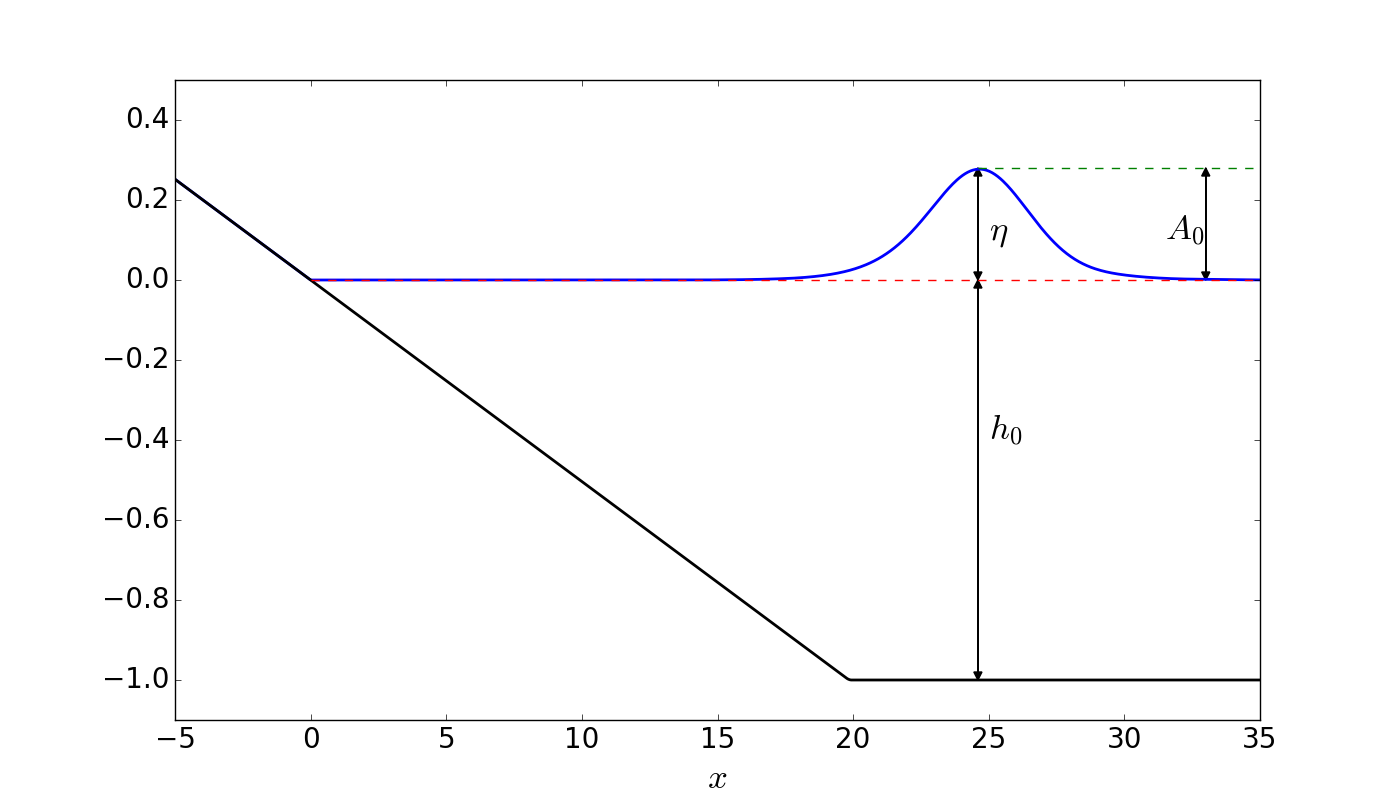
\includegraphics[width=.7\textwidth]{_fig/initial_setup.png}
\caption{Set-up of a numerical test for Synolakis' experiments.}
\label{fig:init_setup}
\end{figure}

In this work, the main interests lie 
with the breaking wave cases, and 
one of the cases in Synolakis (1987) experiments is  
a solitary wave of $A/h=0.28$ approaching a slope of $1:19.85$.
In Figure \ref{fig:init_setup}, 
the initial set-up for a test is shown. 


% The BIM solution is in a good agreement with the experiments to the wave break point, 
%The BIM solution can provide detailed time series solution which the laboratory measurements are lack of. 
In Figure \ref{fig:lab_bim}, the laboratory measurements
are shown with the computational results from the BIM model
for a breaking wave case of Synolakis with $A/h=0.28$ and $1:19.85$ slope
at $t^*=15$. The non-dimensional time 
$t^*=t\sqrt{h/g}$ is used 
in accordance with the laboratory experiments.
The results are in good agreement. 

\begin{figure}[!htb]
\centering
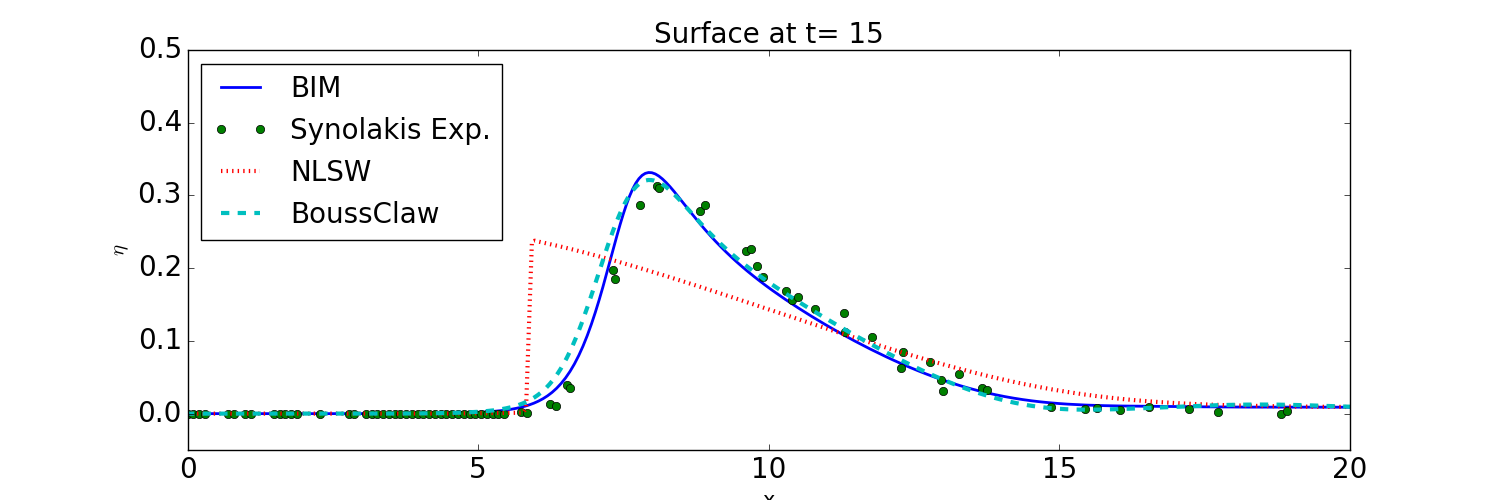
\includegraphics[width=\textwidth]{_fig/lab_bim_t15.png}
\caption{Comparison of the laboratory experiments and BIM at t=15 with $A/h=0.28$ 
on a slope of $1:19.85$.}
\label{fig:lab_bim}
\end{figure}

Figure \ref{fig:bim_breaking} shows
the numerical results from BIM at $t=17$, $18$ and  $18.6$.
In the BIM results a
 vertical front is observed at $x=4.02$ m and $t=18.6$
with the maximum wave amplitude $A=0.414$ m,
and this shows similar results with 
the analysis of Titov and Synolakis (1995) \cite{titov1995modeling}.
\marginpar{\footnotesize What is the esult of Titov and Synolakis?} 
%and the undisturbed depth is $h=0.206$ m. 
The ratio of amplitude to depth, $A/h$, 
is about $2.01$ at the break point.
The potential flow model cannot be run much beyond the
breaking points (until attachment of the plunger only) and 
gives no information on the following  bore propagation.
In Figure \ref{fig:sw_timeseries}, 
computations of the NLSW equations (present model without the second 
fractional step) display a premature bore formation which checks the
amplification during the subsequent shoaling. 
As a consequence the amplitude in the NLSW simulation is markedly smaller than that of the 
potential flow model when the latter indicates breaking.


\begin{figure}[!htb]
\centering
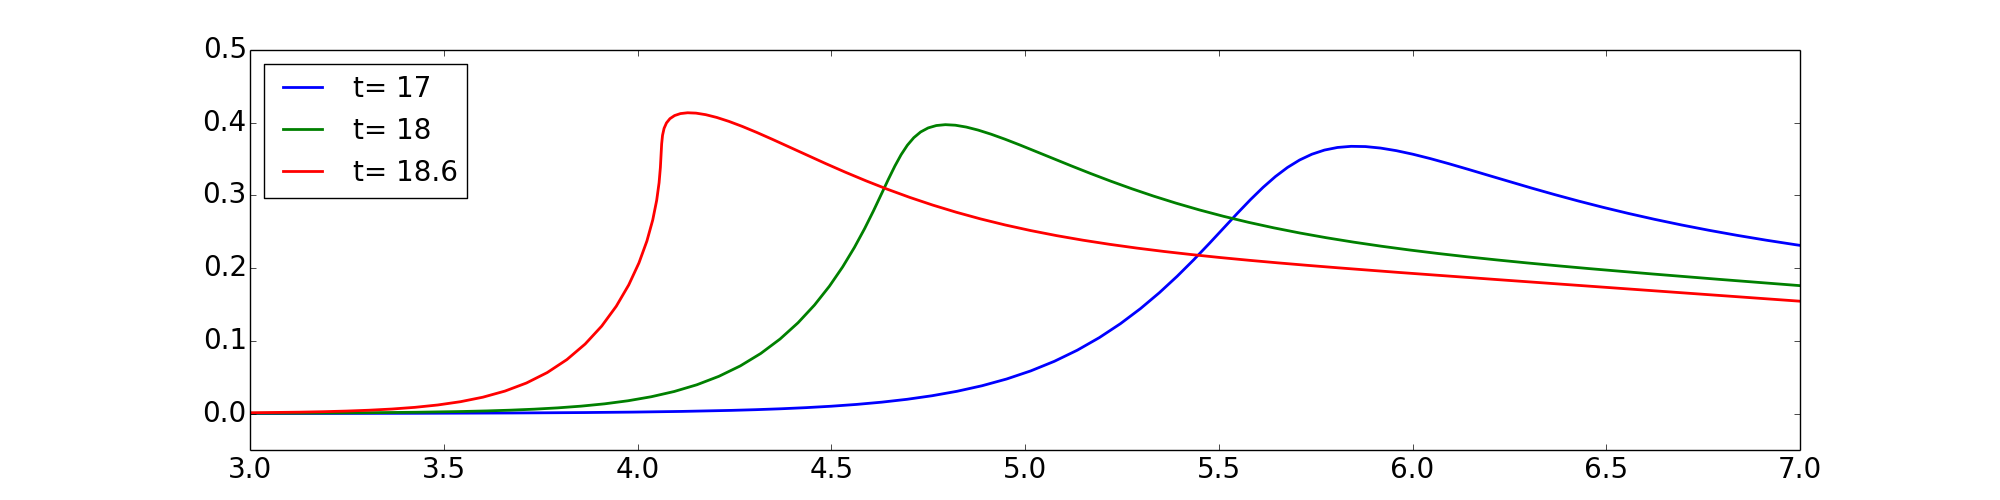
\includegraphics[width=\textwidth]{_fig/bim_n7_time_series.png}
\caption{Computational results from BIM of a wave with $A/h=0.28$ 
on a slope of $1:19.85$.
A vertical front is observed at $t=18.6$. }
\label{fig:bim_breaking}
\end{figure}

%The computation of BIM can not proceed further after $t=19.2$ because of the singularity.

%One of the main reasons is to exclude the effect of the bottom friction. Without appropriate inclusion of the friction forces, the numerical results will not yield comparable results with the experiments. When different numerical models are compared, however, it is difficult to distinguish the friction errors from the modeling errors. Therefore, the numerical solution of BIM without any friction is considered as a solution.

%Figure \ref{fig:sw_timeseries} and \ref{fig:bous_timeseries} show the computational results from depth-averaged models, and both models do not capture the wave breaking properly.
%In Figure \ref{fig:bous_timeseries}, the numerical results from the \textsc{WaveClaw} are given, the amplitude of the incoming wave continues to increase and the wave does not break. 

\begin{figure}[!htb]
\centering
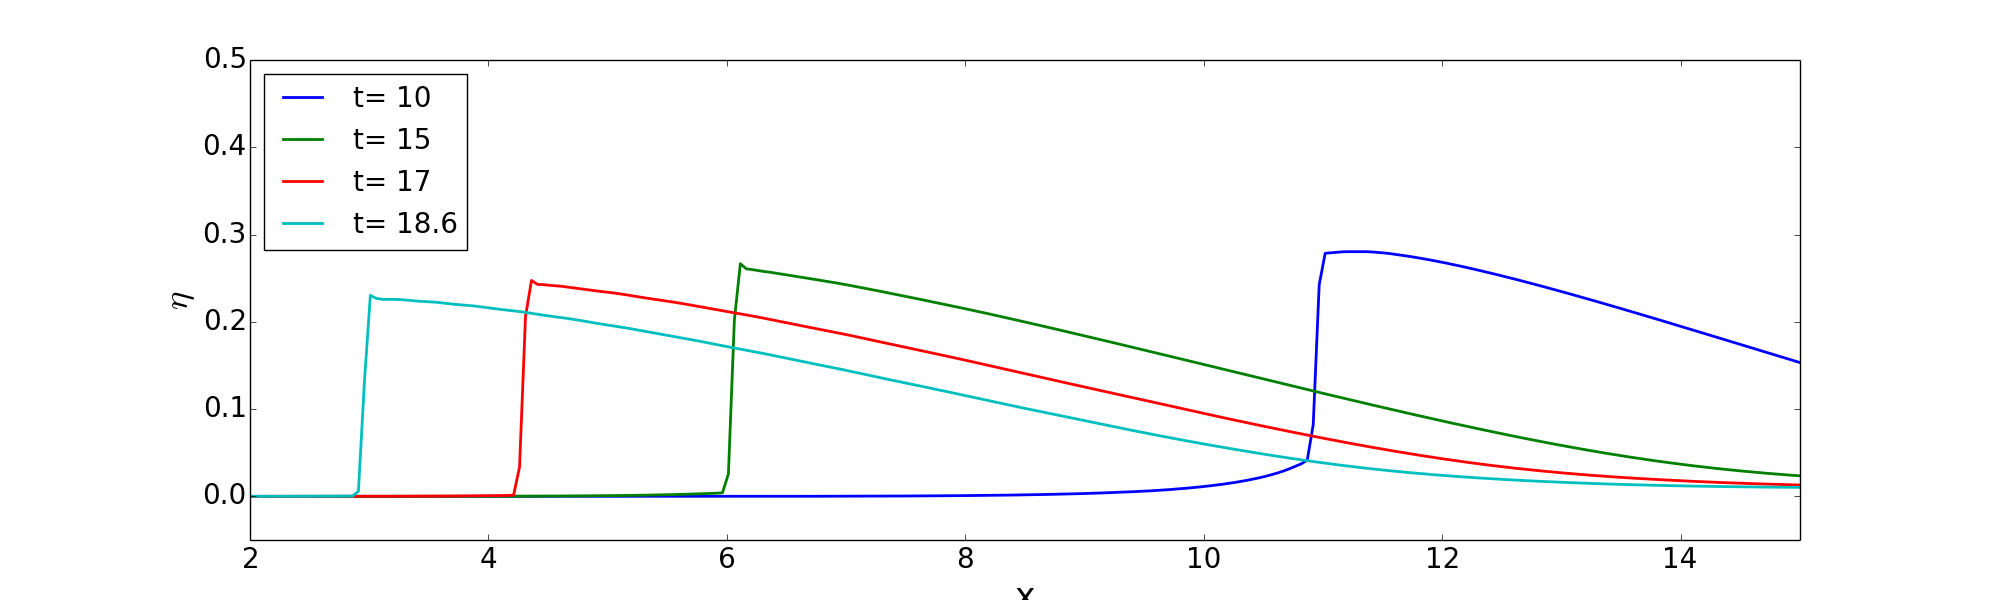
\includegraphics[width=\textwidth]{_fig/sw_dx05_time_series.png}
\caption{Computational results from SWE at $t=10,15,17$ and $18.6$ .  }
\label{fig:sw_timeseries}
\end{figure}

%\begin{figure}[!htb]
%\centering
%\includegraphics[width=\textwidth]{_fig/bous_dx025_time_series.png}
%\caption{Computational results from \textsc{WaveClaw} 
%at $t= 5,9,13,17$ and $20$ s.  }
%\label{fig:bous_timeseries}
%\end{figure}

In their original formulation, 
the Boussinesq-type equations do not take into account 
the post-breaking motion.
In order to combine breaking with  the Boussinesq-type equations
several strategies have been suggested. 
For example, 
Peregrine (1967) \citep{peregrine1967long} used $A/h=0.6$ 
as the break threshold, and also pointed out that
this value reaches around $2$ in some cases of laboratory experiments. 
Shi et. al (2012) \citep{shi2012high} used 
$A/h = 0.8$ as the threshold 
for \textsc{Funwave} based on the Froude analysis 
by Tonelli and Petti (2009) \citep{tonelli2009hybrid}.
Sch{\"a}ffer et al. (1993) \cite{schaffer1993boussinesq} 
introduced the concept of the {\em surface roller}.
Lynett (2006) \cite{lynett2006nearshore} 
investigated $\eta_t/c$, $\eta_x$, $u_{s_{xx}} H^2/c$, and $u_s/c$, 
where $c=\sqrt{gH}$ and $u_s$ = free surface speed,
and then identified that the critical front slope ($\eta_x$) 
is the least sensitive breaking threshold. 
Tissier et al. (2012) \cite{tissier2012new} suggested
a breaking decision model based on the surface roller,
the maximal front angle and the Froude number.
% One of the common drawbacks from these models is that they depend on the choice of the parameters which may be sensitive to the results.
%In this work, the threshold for $\epsilon_B$ will be used.  
L{\o}vholt et al. (2013) performed comprehensive numerical tests
with different operational wave models, 
and studied the capability and limitation of 
the depth-integrated models. 
Matsuyama et al. (2007) \cite{matsuyama2007study} performed experiments
of the wave propagation on various slope angles. 
They studied the wave breaking criteria and suggested 
\begin{align*}
\frac{u_s}{c} = \frac{\eta}{H} - \frac{h}{3H}
\left(
H\frac{\partial^2 \eta}{\partial x^2} - 2 \left(\frac{\partial \eta}{\partial x} \right)^2
\right),
\end{align*}
as a wave breaking criterion.

Although several criteria for the wave break have been suggested,
it needs further studies to determine which criteria are more accurate.
It should be noted 
that the criteria are sensitive, and 
the same value may not be applied 
to other wave models in different wave experiments.
At the same time, the computational efficiency and implementation
should be considered in the wave break models. 

\section{Numerical Tests}

\subsection{Solitary wave propagation}

In order to validate the numerical approach 
a solitary wave propagation is tested on a constant water depth.
For the initial conditions, 
the analytic solitary wave solution 
of the Serre's equations is used
since analytic solutions are unknown 
for
the set (\ref{eq:madsen_cons_mass}) and 
(\ref{eq:madsen_momx}).
Solitary wave solutions to the Serre's equations are given as
\begin{flalign}
\label{eq:anal_serre}
\begin{split}
& \eta(x,t) = A \textrm{sech}^2 \left( \kappa (x-ct)\right),  \\
& u(x,t) = c \frac{\eta(x,t)}{h},
\end{split} &
\end{flalign}
where
\begin{flalign}
\begin{split}
& \kappa = \frac{\sqrt{3h}}{2A\sqrt{A+h}}, \quad \textrm{and}
 \quad c = \sqrt{g\left( A + h \right)}.
\end{split} &
\end{flalign}
In this expression, $A$ and $h$ are constants
which represent the wave amplitude and the undisturbed water depth
respectively,
and this solution is only valid for a constant water depth.

In Figure \ref{fig:soliton_ts}, 
snapshots from the \textsc{WaveClaw}'s simulation is shown 
at $t=0,4,8$ and $12$ s with $\Delta x = 0.1$. 
For the initial conditions, the solution \ref{eq:anal_serre}
is used with $A=0.2$, $h=1$ and $g=9.81$.
The computational results are in a good agreement 
with the analytic solutions concerning height, shape and propagation speed. 
The amplitudes decreases very gently as the wave propagates. 
The discreapancy may be  partially due to the numerical errors
and partly to the fact that 
the analytic solution for Serre's equations satisfies
the present Boussinesq-type equations only approximately.

\begin{figure}[!htb]
\centering
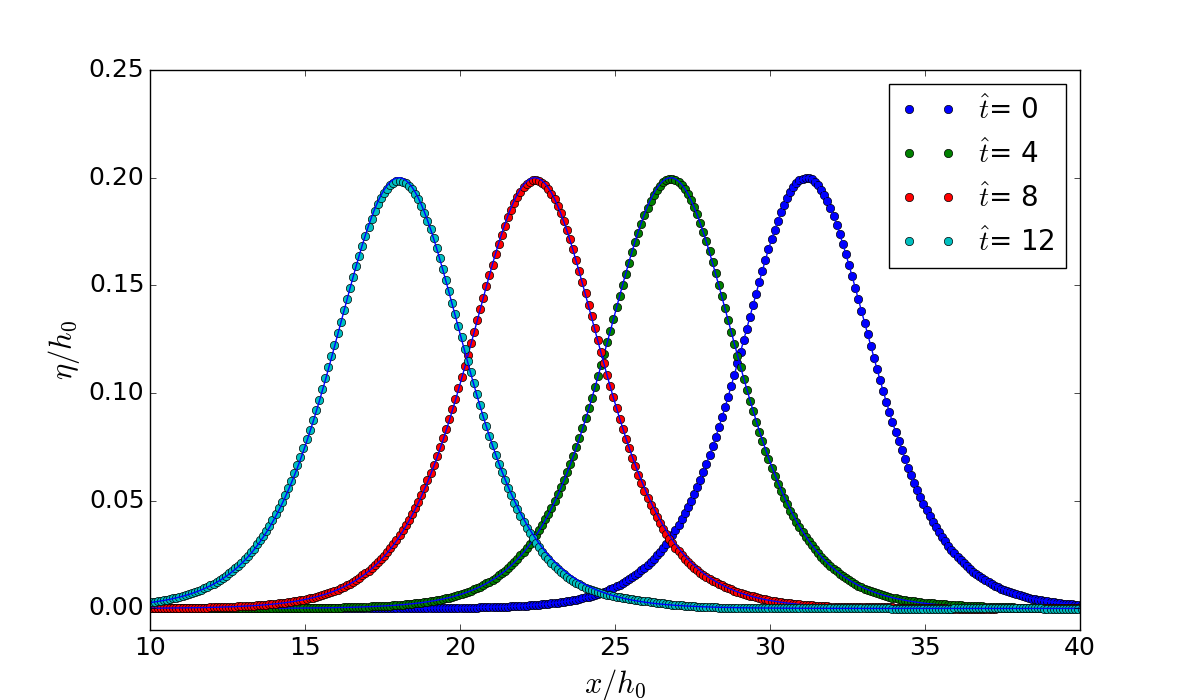
\includegraphics[width=.8\textwidth]{_fig/soliton_ts.png}
\caption{Snapshot of the analytic and computed solitary wave 
at $t=0,4,8$ and $12$ with $A/h=0.2$. 
The wave propagates from right to left,
and the analytic solutions are black solid lines.}
\label{fig:soliton_ts}
\end{figure}

In Figure \ref{fig:soliton_error},
the relative error of the maximum amplitude at $t=12$,
\begin{flalign*}
E_{\infty} = \frac{\left| A_{comp}-A_{sol} \right|}{A_{sol}}, &
\end{flalign*}
is shown for $\Delta x$.
The relative error for $A/h=0.05$ is smaller 
than $A/h=0.2$
because it is assumed that $A/h$ is small 
in the derivation of the Boussinesq equations.

\begin{figure}[!htb]
    \centering
    \begin{subfigure}[b]{0.45\textwidth}
        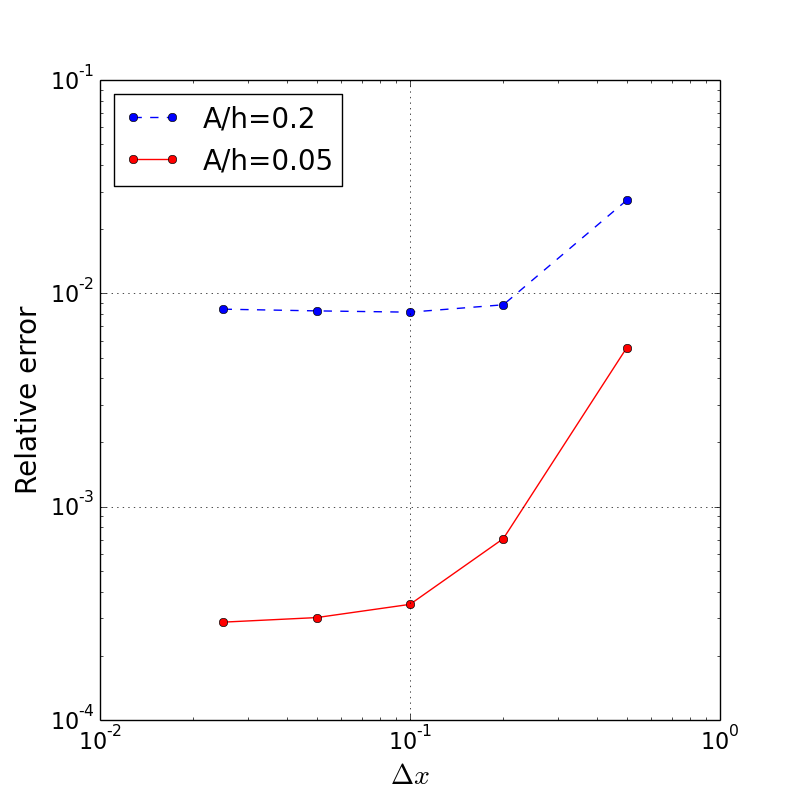
\includegraphics[width=\textwidth]{_fig/soliton_error.png}
        \caption{Relative error of max. amplitude}
        \label{fig:soliton_error}
    \end{subfigure}
    \begin{subfigure}[b]{0.45\textwidth}
        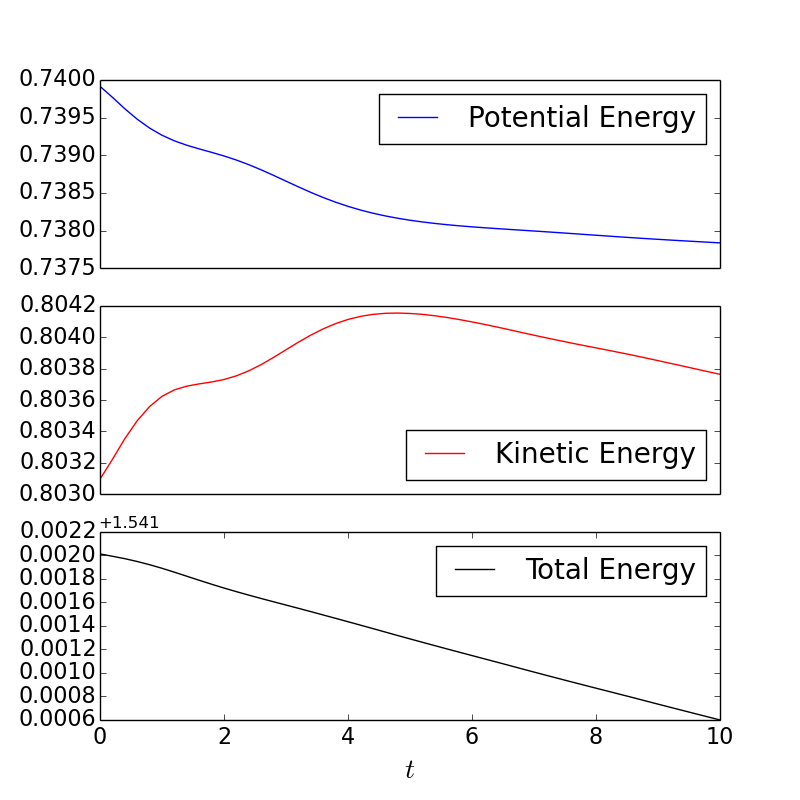
\includegraphics[width=\textwidth]{_fig/soliton_energy.png}
        \caption{Energy}
        \label{fig:soliton_energy}
    \end{subfigure}
    \caption{Relative error and energy of a soliton on a constant depth.}
    \label{fig:soliton_error_energy}
\end{figure}

The wave energies for the NLSW and the Boussinesq equations are $E_0$ and $E_0+E_1$, respectively, where
\begin{flalign}
& E_0 = \frac{1}{2}\left( g\eta^2 + H\bar{u}^2 \right), \label{eq:energy_e0} \\
& E_1 = \frac{1}{6}H^3\bar{u}_x^2
+ \frac{1}{2}H^2h_x\bar{u}\bar{u}_x + \frac{1}{2}Hh_x^2\bar{u}^2.
\label{eq:energy_e1}
\end{flalign}
Details are given in  Madsen et al. (1997) \citep{madsen1997surf} 
and \ref{append:energy}, for example.

%The wave energy is conserved 
%as long as the wave is smooth and do not break,
%and the energy decreases as the wave breaks.
%The energy can be divided into the potential energy and kinetic energy, and the potential energy of $E_0+E_1$ is $\frac{1}{2} g\eta^2$.
In Figure \ref{fig:soliton_energy}, the energy of the solitary
wave is shown with $A/h=0.2$, and both the potential and kinetic energy
remain constant, showing that the numerical procedure has negligible
 dissipation for smooth wave shapes.


\subsection{Waves on a composite slope}

A physical model was constructed at the Coastal Hydraulic Laboratory of the U.S. Army Corps of Engineers
in order to address beach erosion and severe flooding problems.
The description of the benchmark problem can be found
at CHL webpage \cite{chl_bp5}.
The model beach consists of three piecewise linear slopes of 1:53, 1:150, and 1:13 with a vertical wall at the shoreline as shown in Figure \ref{fig:bp5_water_tank}.
In the laboratory, the wavemaker was located at 23.23 m.
The gauge data from three cases are provided 
where the ratio $A/h$ is equal to $0.038$, $0.259$ and $0.681$
with $h=21.8$ cm.

\begin{figure}[!htb]
\centering
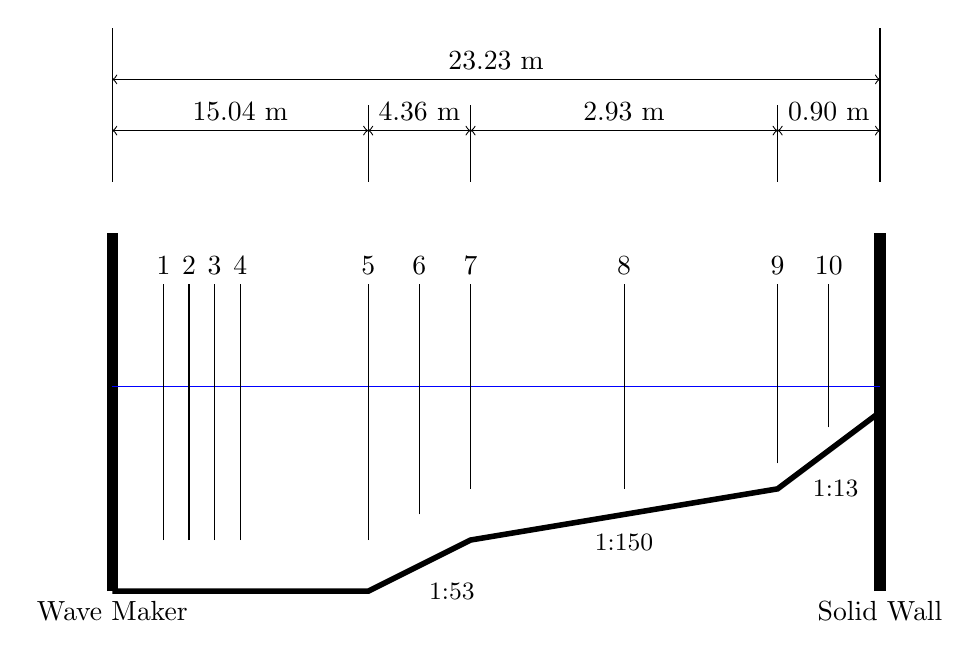
\begin{tikzpicture}[scale=.65]
 \draw[line width=4pt] (0,-4) -- (0,3);
 \draw[line width=2pt] (0,-4) -- (5,-4) -- (7,-3) --(13,-2) -- (15,-0.5);
 \draw[line width=4pt] (15,-4)--(15,3);
 \node[below] at (0,-4) {Wave Maker};
 \node[below] at (15,-4) {Solid Wall};
 \draw[blue] (0,0) -- (15,0);
 \draw (1,-3) -- (1,2) node[above]{1};
 \draw (1.5,-3) -- (1.5,2) node[above]{2};
 \draw (2,-3) -- (2,2) node[above]{3};
 \draw (2.5,-3) -- (2.5,2) node[above]{4};
 \draw (5,-3) -- (5,2) node[above]{5};
 \draw (6,-2.5) -- (6,2) node[above]{6};
 \draw (7,-2) -- (7,2) node[above]{7};
  \draw (10,-2) -- (10,2) node[above]{8};
 \draw (13,-1.5) -- (13,2) node[above]{9};
 \draw (14,-0.8) -- (14,2) node[above]{10};
 \node[right] at (6,-4) {\small 1:53};
 \node[below] at (10,-2.7) {\small 1:150};
 \node[right] at (13.5,-2) {\small 1:13};
 \draw (0,4) -- (0,7);
 \draw (15,4) -- (15,7);
 \draw[<->] (0,6) -- (15,6);
 \node[above] at (7.5,6) {23.23 m};
 \draw[<->] (0,5) -- (5,5);
 \node[above] at (2.5,5) {15.04 m};
 \node[above] at (6,5) {4.36 m};
 \draw[<->] (5,5) -- (7,5);
 \node[above] at (10,5) {2.93 m};
 \draw[<->] (7,5) -- (13,5);
 \draw[<->] (13,5) -- (15,5);
 \node[above] at (14,5) {0.90 m};
 \draw (5,4) -- (5,5.5);
 \draw (7,4) -- (7,5.5);
 \draw (13,4) -- (13,5.5);
  \end{tikzpicture}
  \caption{A sketch of the water tank}
  \label{fig:bp5_water_tank}
\end{figure}

The second case with $A/h=0.259$ have been 
compared with the numerical tests
which were solved on a $400$ point grid with no friction.
%And the switching scheme between the shallow water equations and the Boussinesq equations, is not applied.
To specify the incoming wave from the left boundary, 
the data at Gauge 4 were used for the wave height,
and the corresponding velocity (\ref{eq:anal_serre})
was applied.

In Figure \ref{fig:bp5b_gauges}, water surface elevations
at the gauge 5, 7 and 8 are shown for $A/h=0.269$ case. 
For the incoming waves, the agreement 
between the laboratory measurements and numerical simulations is good. 
For the reflecting waves, some differences are observed,
Because the depth-averaged model is not capable 
of describing the full interaction between the wave and the wall
at the right boundary.\marginpar{\footnotesize Geir: A very shallow region may yield important frictional effects? But, surely, the wave should  break in the shallowest region?}
 
Friction forces are not applied in the numerical simulation
which may become important at the shallow region. 
Although a difference in the wave speed is observed,
the general wave pattern is well captured. 

\begin{figure}[!htb]
\centering
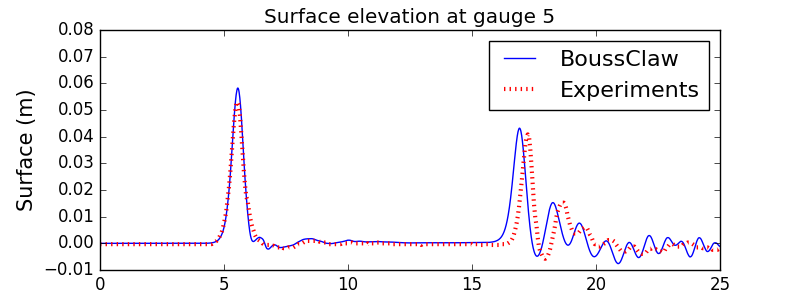
\includegraphics[width=.8\textwidth]{_fig/gauge0005fig300.png}\\
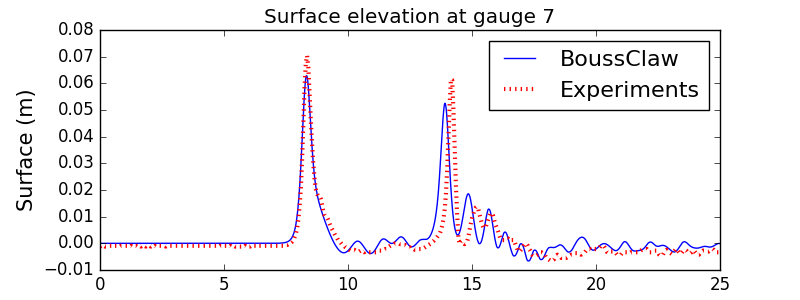
\includegraphics[width=.8\textwidth]{_fig/gauge0007fig300.png}\\
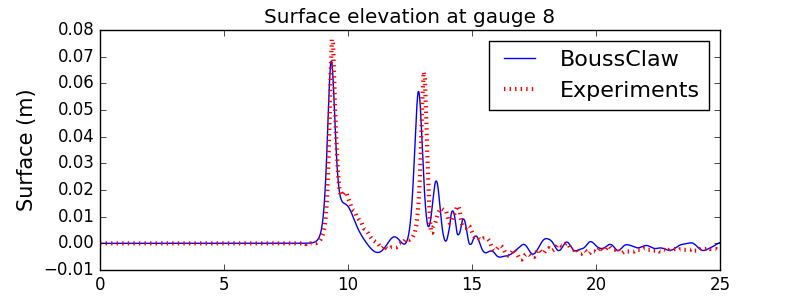
\includegraphics[width=.8\textwidth]{_fig/gauge0008fig300.png}
\caption{Water surface elevation at gauges 5,7 and 8 for $A/h=0.269$ case.}
\label{fig:bp5b_gauges}
\end{figure}

\section{Breaking waves on a slope}

The set-up of the wave tank follows 
the laboratory experiments by Synolakis (1987) \citep{synolakis1987runup}. 
The wave tank is assumed to have one horizontal direction,
and the bathymetry is composed of a horizontal bottom and 
a uniform slope as shown in Figure \ref{fig:init_setup}. 
A solitary wave of $A/h=0.28$ is generated at the right side
and propagates to the shore on the left side. 

In the measurement of Synolakis (1987), $t=0$ was set 
when the distance from the wave crest to the toe of the slope is equal to $L$,
where $L$ is given as
\begin{flalign*}
& L = \sqrt{\frac{4A}{3h}} \textrm{arccosh} \left( \frac{1}{0.05} \right). &
\end{flalign*}
When $t=0$, however, the solitary wave then has an elevation of
5\% of it maximum at the toe of the beach. 
This is too much in a modeling context.  
Instead, the solitary solution (\ref{eq:anal_serre}) 
is imposed at $L + 5c$
so that the initial wave is on a horizontal bottom. 
%Then $t=0$ is set as soon as the peak of wave is at $x=L$.

\iffalse

As the wave approaches the shoreline,
the wave amplitude increases and the wavelength shortens. 
In numerical simulations,
the grid size should be small enough 
to be able to capture the short wavelength 
In Figure \ref{fig:dgeo_grids}, 
the computational results at t=$18$, $20$ and $22$ are shown 
with grid size $\Delta x = 0.025, 0.05$ and $0.1$ m. 
When the wave is smooth at $t=18$, the different grid sizes
show similar results. 
As the wave approaches the shoreline,
the wave amplitude increases and the wavelength shortens. 
At t=$22$ , the wave is condensed,
and the wavelength is shortened.
Thus small grid $\Delta x=0.025$ is necessary 
in order to capture the wave steepening properly at t=$22$.

\begin{figure}[!htb]
\centering
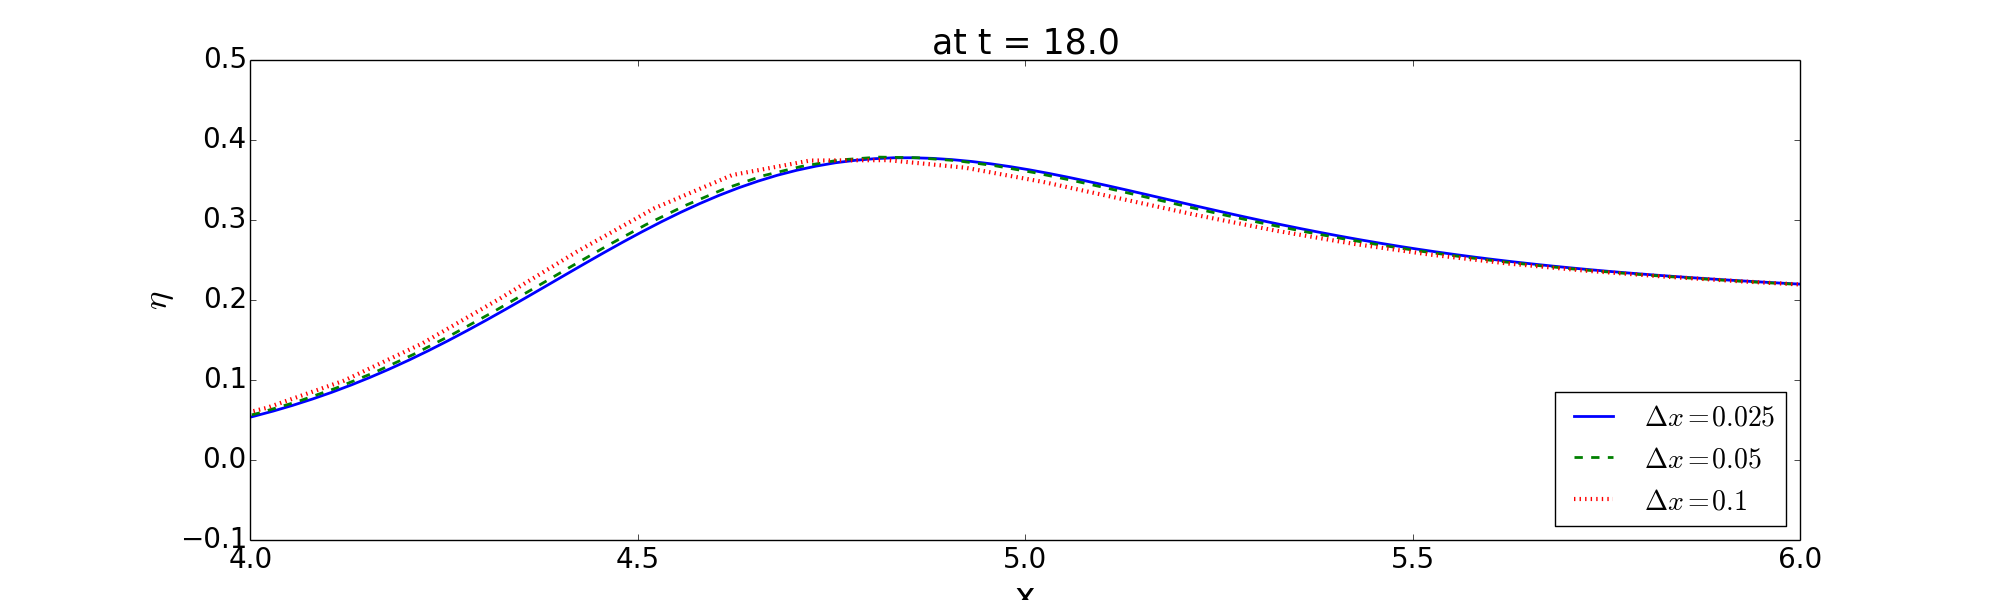
\includegraphics[width=.9\textwidth]{_fig/dgeo_grids_t18.png}\\
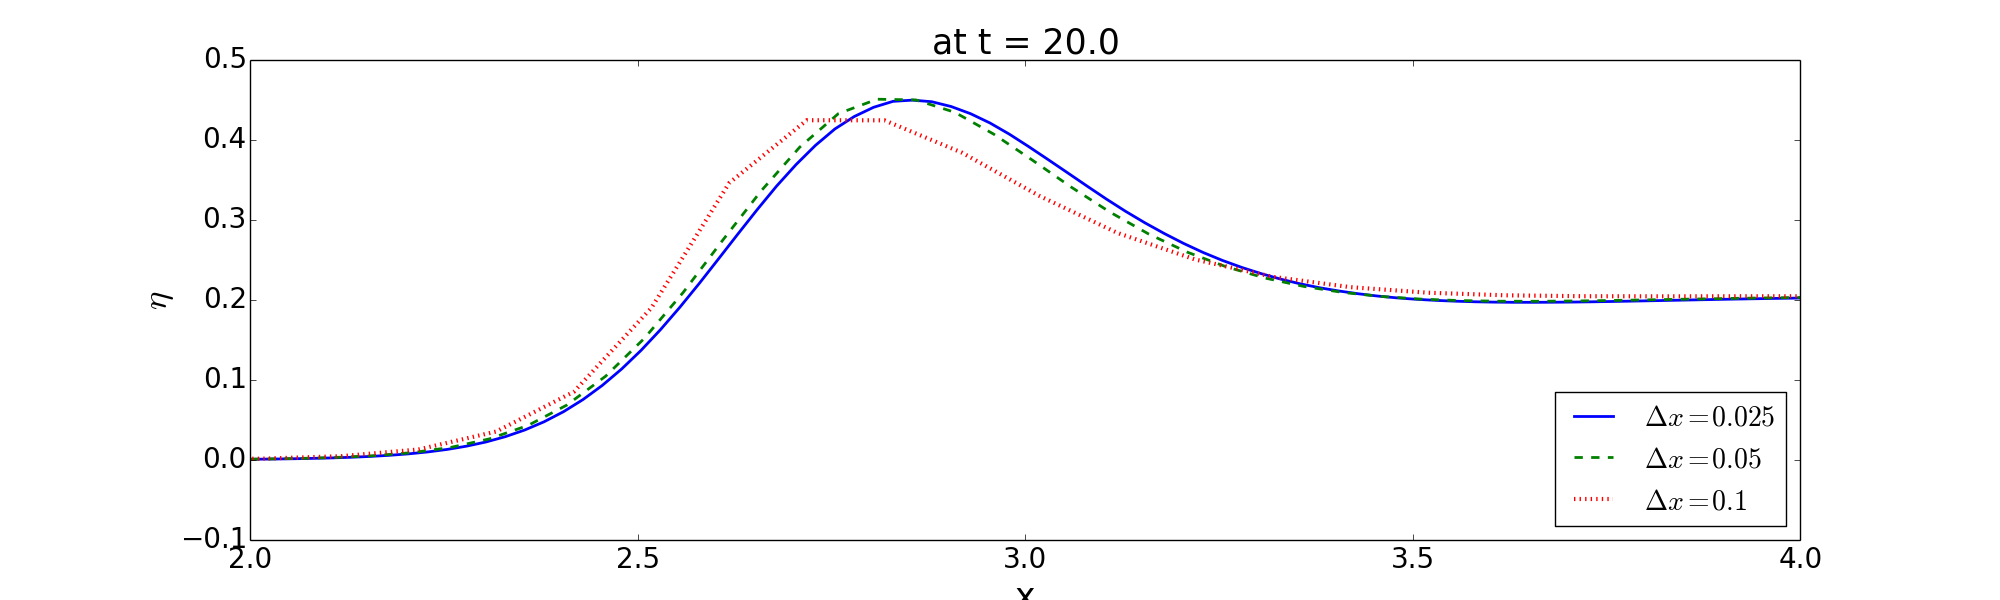
\includegraphics[width=.9\textwidth]{_fig/dgeo_grids_t20.png}\\
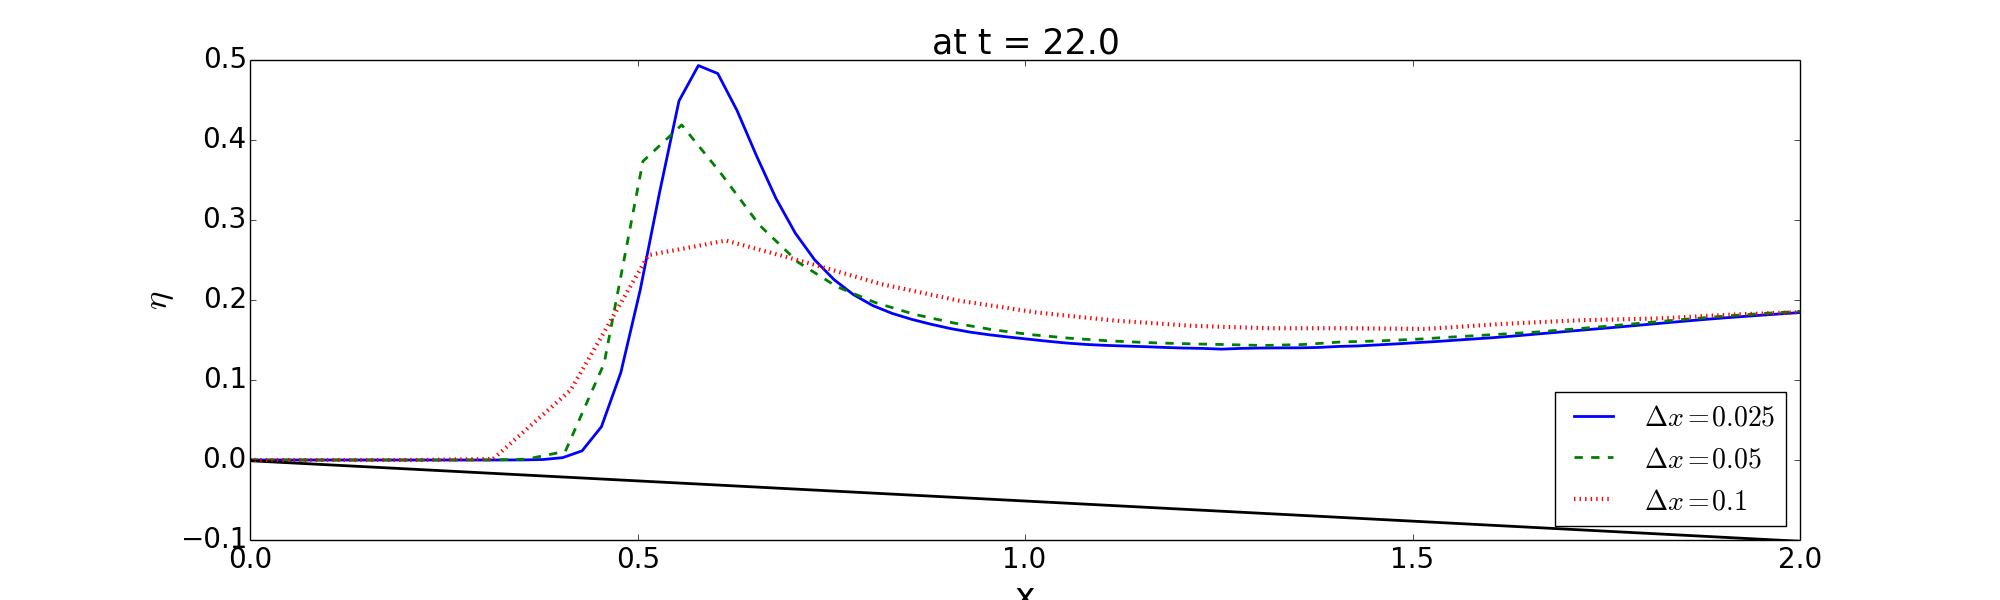
\includegraphics[width=.9\textwidth]{_fig/dgeo_grids_t22.png}
\caption{Snapshot of the \textsc{WaveClaw} results 
at t=$18$, $20$ and $22$
with $\Delta x=0.025$, $0.05$ and $0.1$ m.}
\label{fig:dgeo_grids}
\end{figure}

\fi

Figure \ref{fig:bim_dgeo} shows the snapshots of 
the water surface at t=$16, 18,$ and $18.6$
from BIM and \textsc{WaveClaw} with B=$0$ and $1/15$.
When the wave is smooth at t=16, the \textsc{WaveClaw}
results are almost identical. 
At the break point, $t=18.6$, larger differences are observed. 
If $B=0$, the wave speed is slightly faster 
than the BIM result, but the wave amplitude is similar. 
When $B=1/15$, the wave speed matches the BIM results better,
but the amplitude is slightly smaller. 
In general, the computational results are rather similar
with $B=0$ and $1/15$. 

\begin{figure}[!htb]
\centering
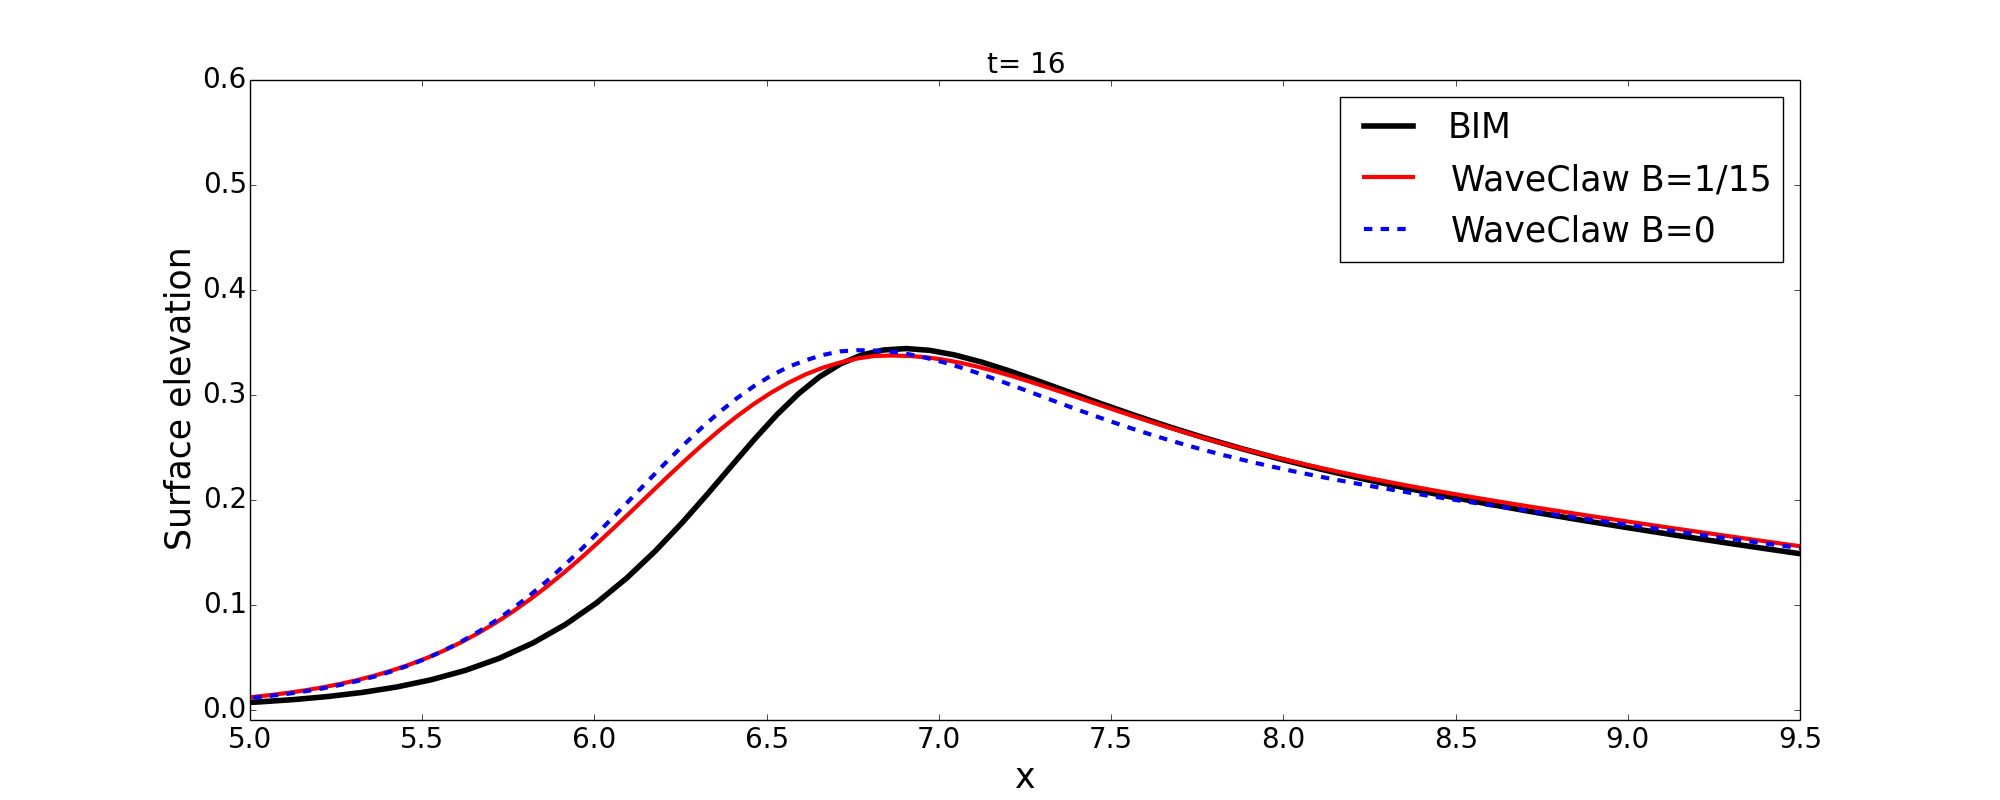
\includegraphics[width=.9\textwidth]{_fig/bim_dgeo_160.png}\\
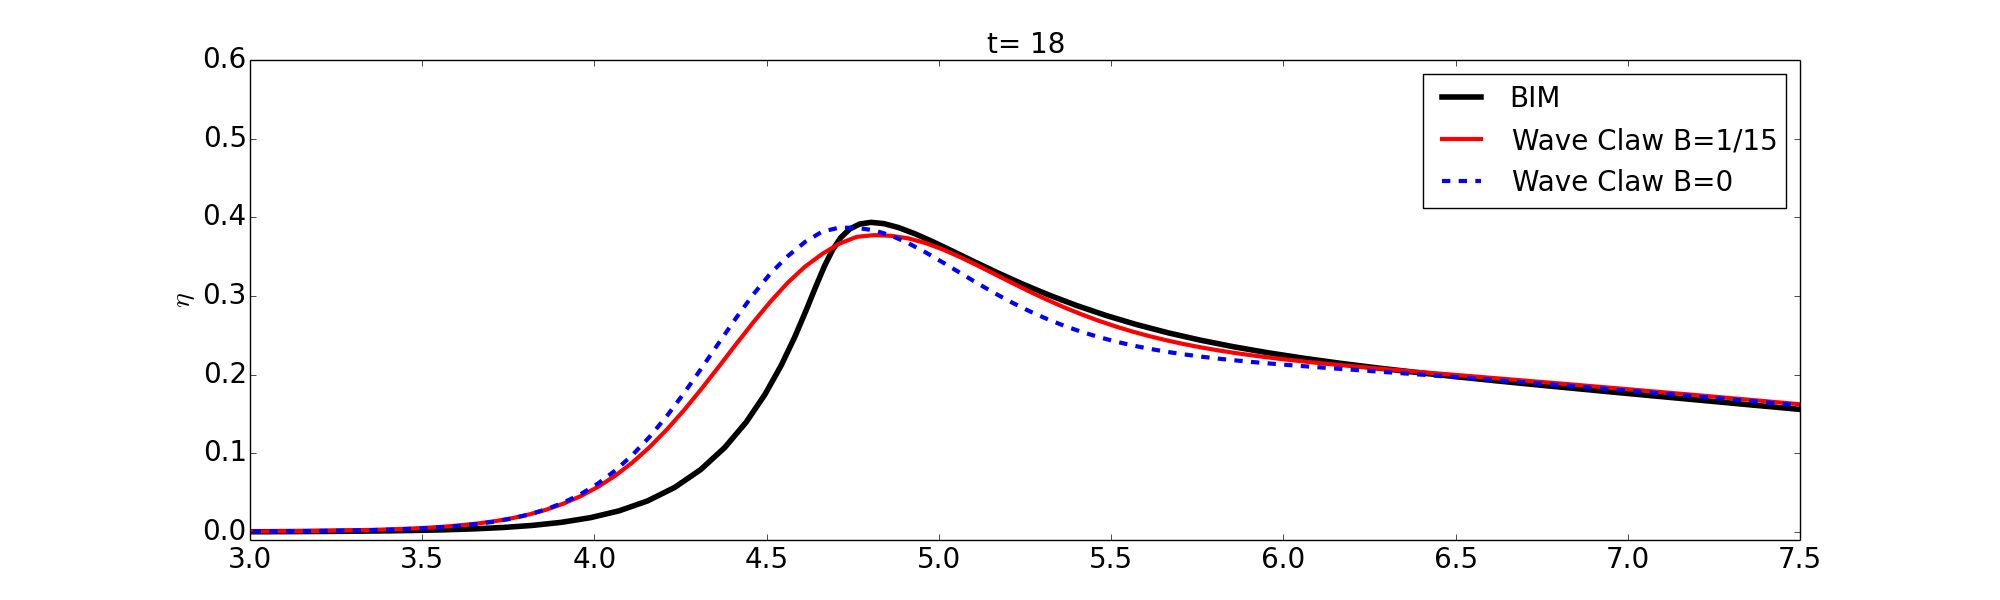
\includegraphics[width=.9\textwidth]{_fig/bim_dgeo_180.png}\\
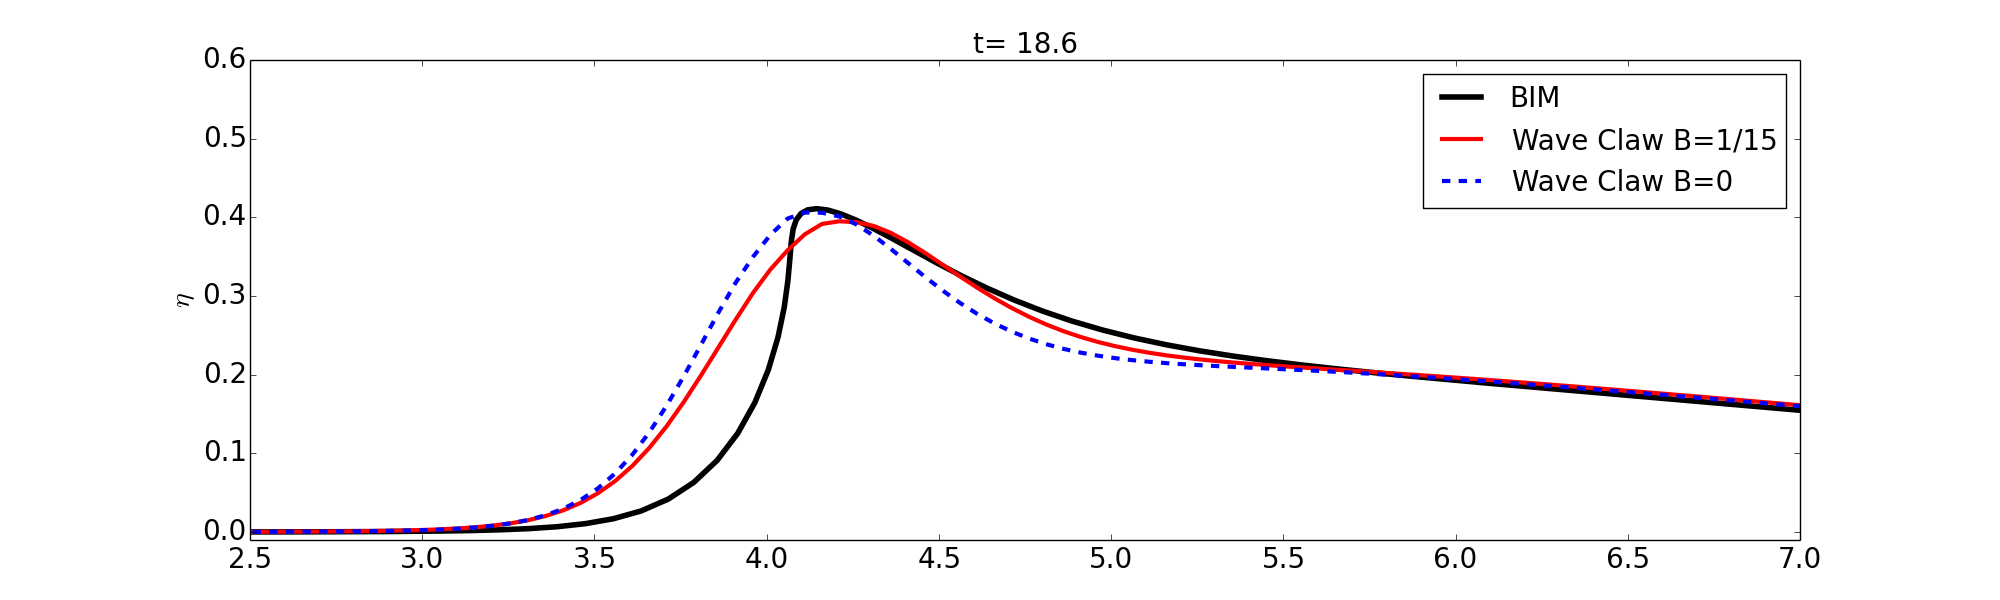
\includegraphics[width=.9\textwidth]{_fig/bim_dgeo_186.png}
%\includegraphics[width=.7\textwidth]{_fig/bim_dgeo_192.png}
\caption{Snapshots of BIM and \textsc{WaveClaw} with B=$0$ and $1/15$ at t=$16$, $18$ and $18.6$.}
\label{fig:bim_dgeo}
\end{figure}

The numerical simulations of 
the \textsc{WaveClaw} are compared
with the pre-existing softwares. 
\textsc{Geoclaw} software \cite{clawpack} is chosen
as a reference to the shallow water equations.
The Boussinesq-type equation solvers
such as \textsc{Funwave} \cite{shi2012high}, \textsc{GloBouss} \cite{lovholt2010coupling} and the Serre type \cite{Lovholt:2013a}, 
have also been used for comparison. . 
In the computations 
the original Serre's equations are enhanced by adding the Sch{\"a}ffer et al. (1995) \cite{schaffer1995further} terms. 
%And the boundary integral method (BIM) for the full potential theory is also considered. 
%The threshold of the wave breaking is not used in this section. 

In Figure \ref{fig:bim_dgeo_fun}, snapshots from different
numerical models are shown at t=$15$, $17$ and $18$. 
At t=$15$, the computational results
from different numerical tools show slightly different results,
but the general pattern is similar.
At t=$17$, some discrepancies are observed into two groups, and
\textsc{GloBouss} and \textsc{Funwave} 
are analogous meanwhile \textsc{WaveClaw}
and Serre's results are alike. 
The wave amplitudes computed by \textsc{GloBouss} and \textsc{Funwave},
are more than 10 \% larger than BIM.
The wave amplitude continues to increase 
with \textsc{GloBouss} and \textsc{Funwave} simulations,
and the difference from the BIM result becomes larger at t = $18$. 
The results from the Serre and \textsc{WaveClaw} models are 
very similar to those of the BIM model. 
Especially, the wave amplitudes are correctly determined by these models.
%\marginpar{\footnotesize Then why don't we use Serre?}

\begin{figure}[!htb]
\centering
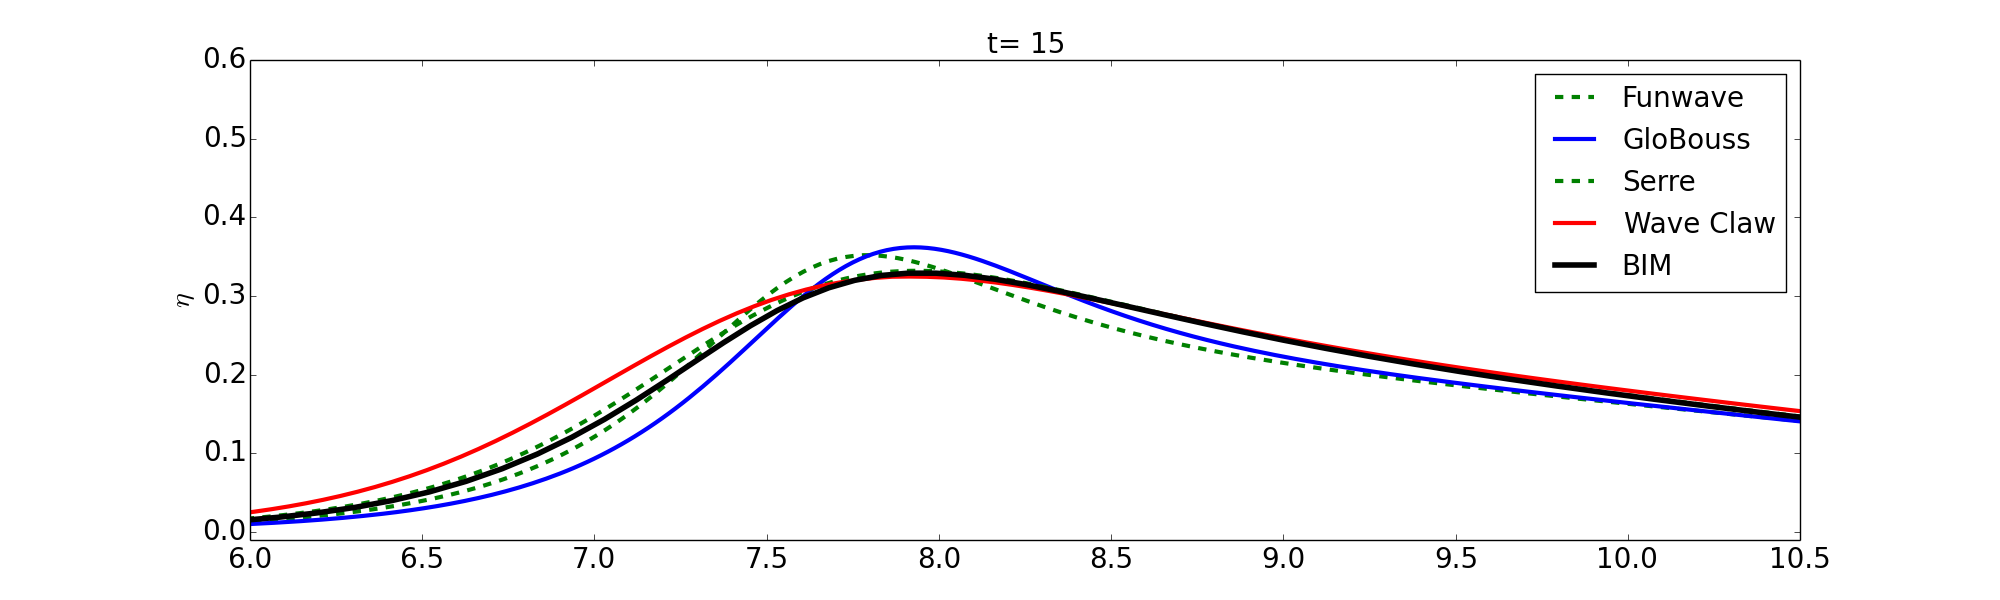
\includegraphics[width=.9\textwidth]{_fig/bim_dgeo_fun_glob_150.png}\\
%\includegraphics[width=.9\textwidth]{_fig/bim_dgeo_fun_glob_160.png}\\
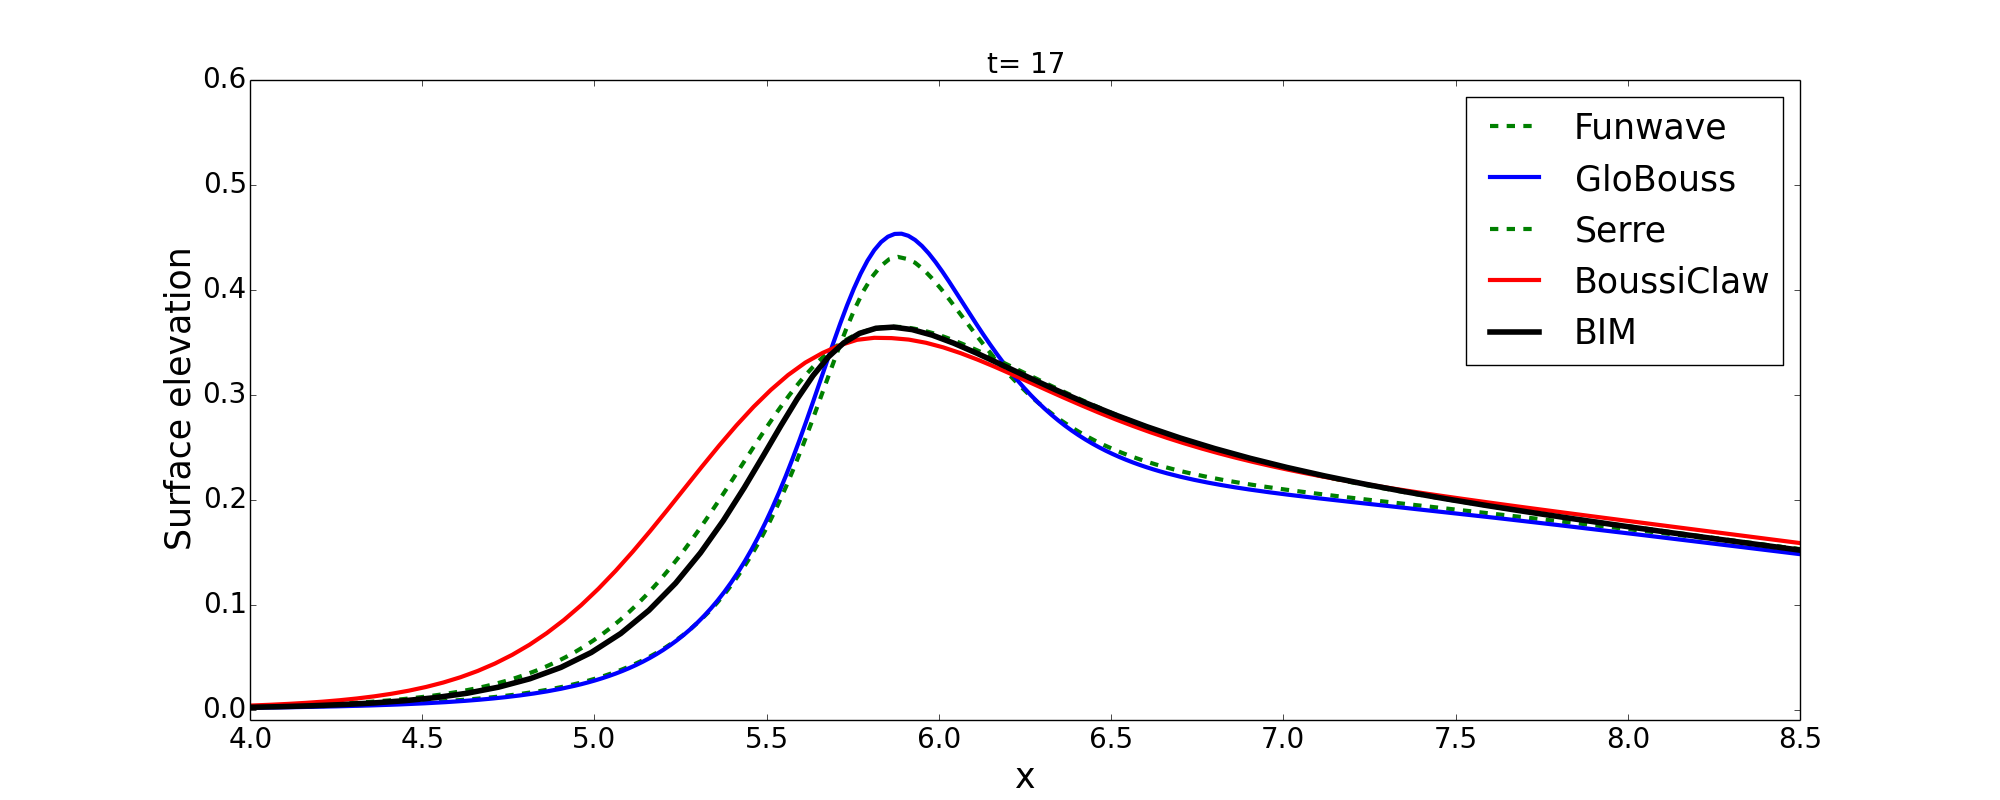
\includegraphics[width=.9\textwidth]{_fig/bim_dgeo_fun_glob_170.png}\\
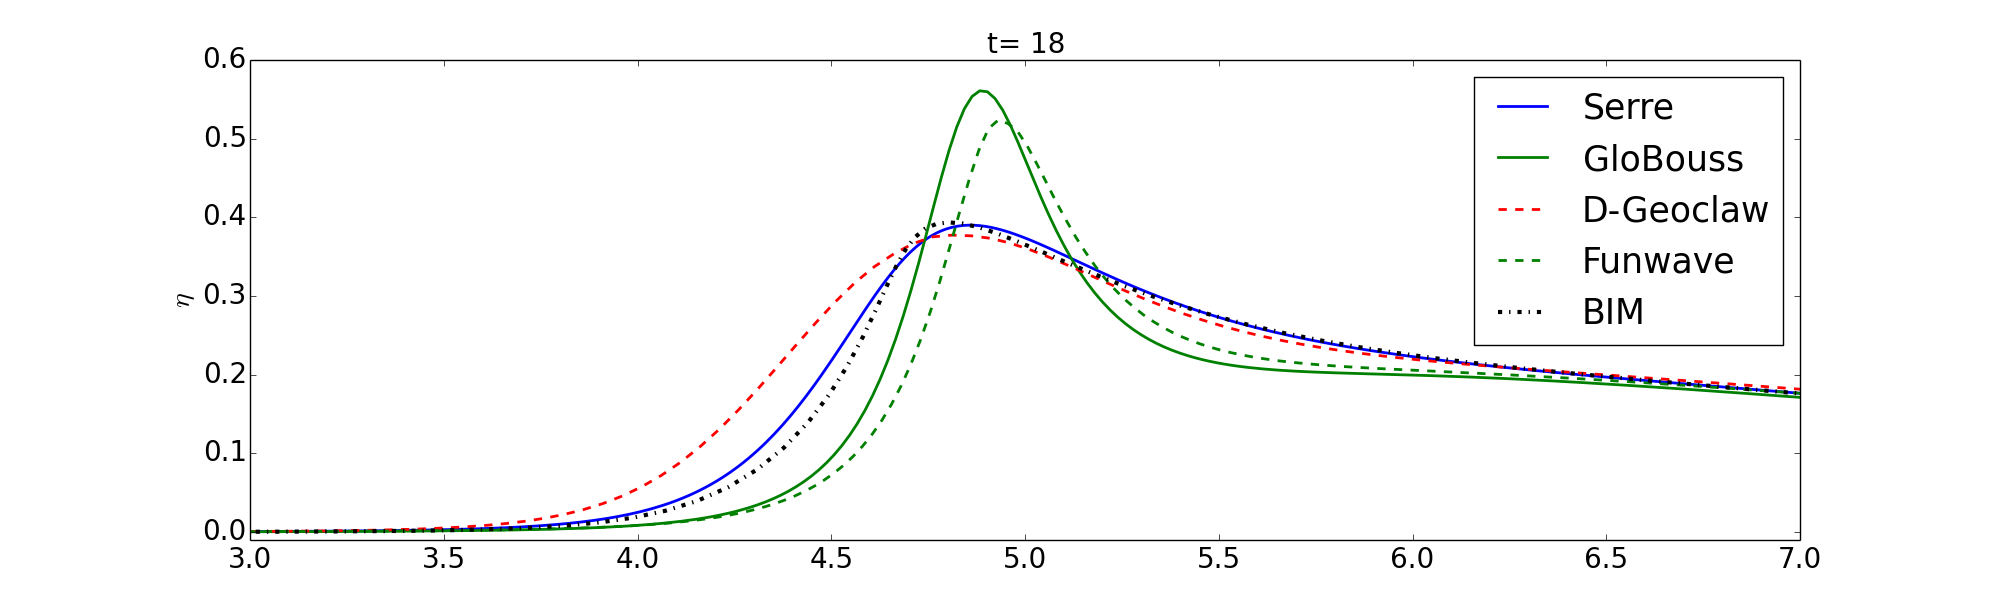
\includegraphics[width=.9\textwidth]{_fig/bim_dgeo_fun_glob_180.png}
\caption{Snapshots of BIM, Serre, \textsc{GloBouss}, \textsc{WaveClaw}
and \textsc{Funwave} at t = $15$, $17$ and $18$.
The \textsc{WaveClaw} is used with B=$1/15$,
and the Peregrine's form is used for \textsc{GloBouss}.}
\label{fig:bim_dgeo_fun}
\end{figure}

\subsection{Wave Breaking}

In order to catch wave breaking in a heuristic fashion,
a threshold on $\epsilon_B:=\eta/h$ is applied to the \textsc{WaveClaw}.
When the threshold is reached, 
the wave breaking is supposed to be initiated, 
and the dispersive terms are suppressed.
At the breaking, the set of equations is
switched to the shallow water equations
in the vicinity of the wave crest.
In the numerical simulation of the \textsc{WaveClaw} model,
the ratio $\epsilon_B$ reaches the threshold $0.8$ at $t=14.9$
when the peak of the wave is at $x=8.03227$ m.
At this time, the wave breaking is assumed to start, 
and the governing equations are switched 
to the shallow water equations.
%Meanwhile, the BIM results show $x=4.02$ m and  $\epsilon_B=2.01$ at the start of the wave breaking.

\begin{figure}[!htb]
\centering
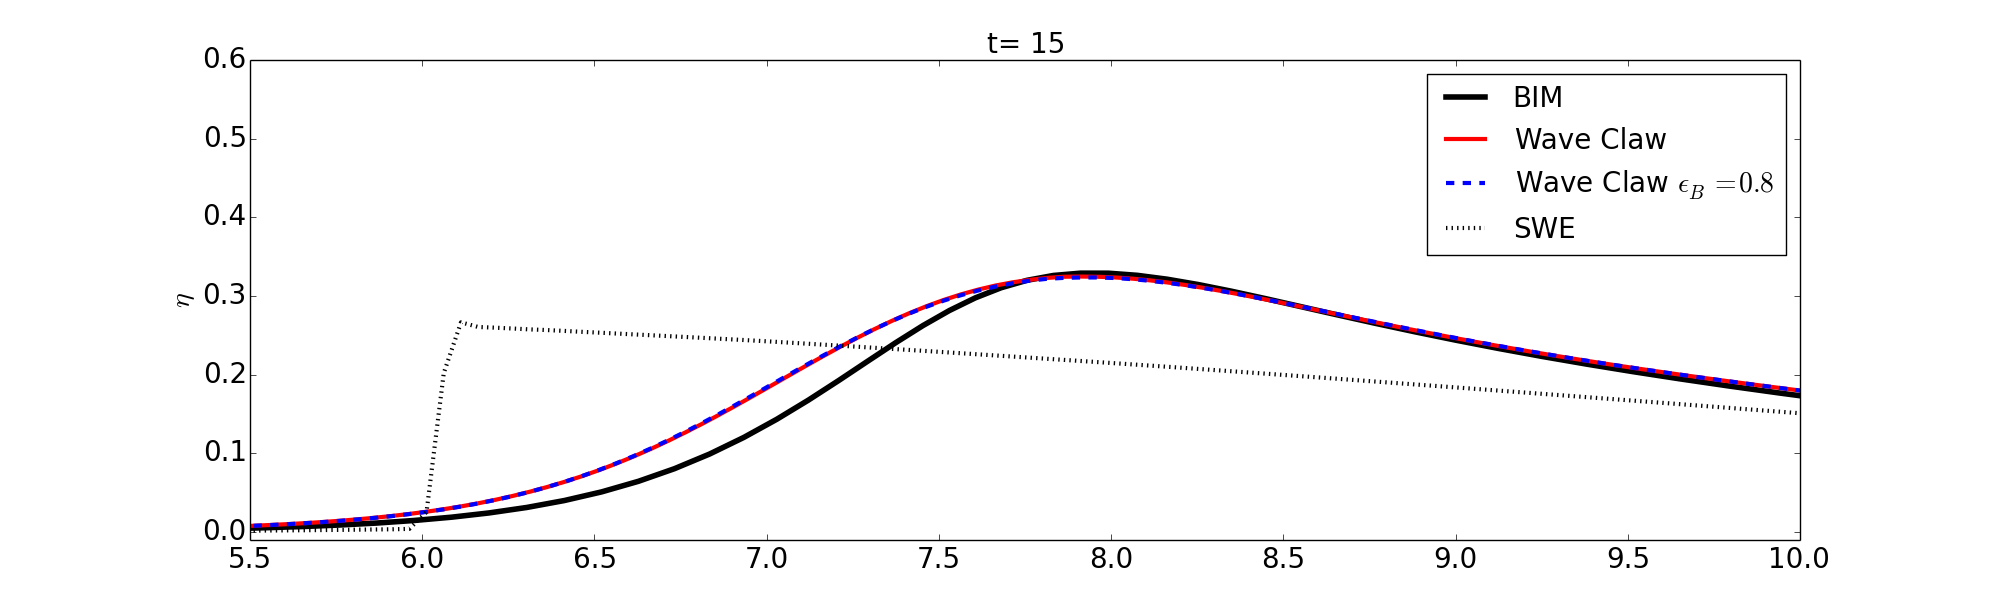
\includegraphics[width=.9\textwidth]{_fig/bim_dgeo_etaB8_150.png}\\
%\includegraphics[width=.9\textwidth]{_fig/bim_dgeo_etaB8_160.png}\\
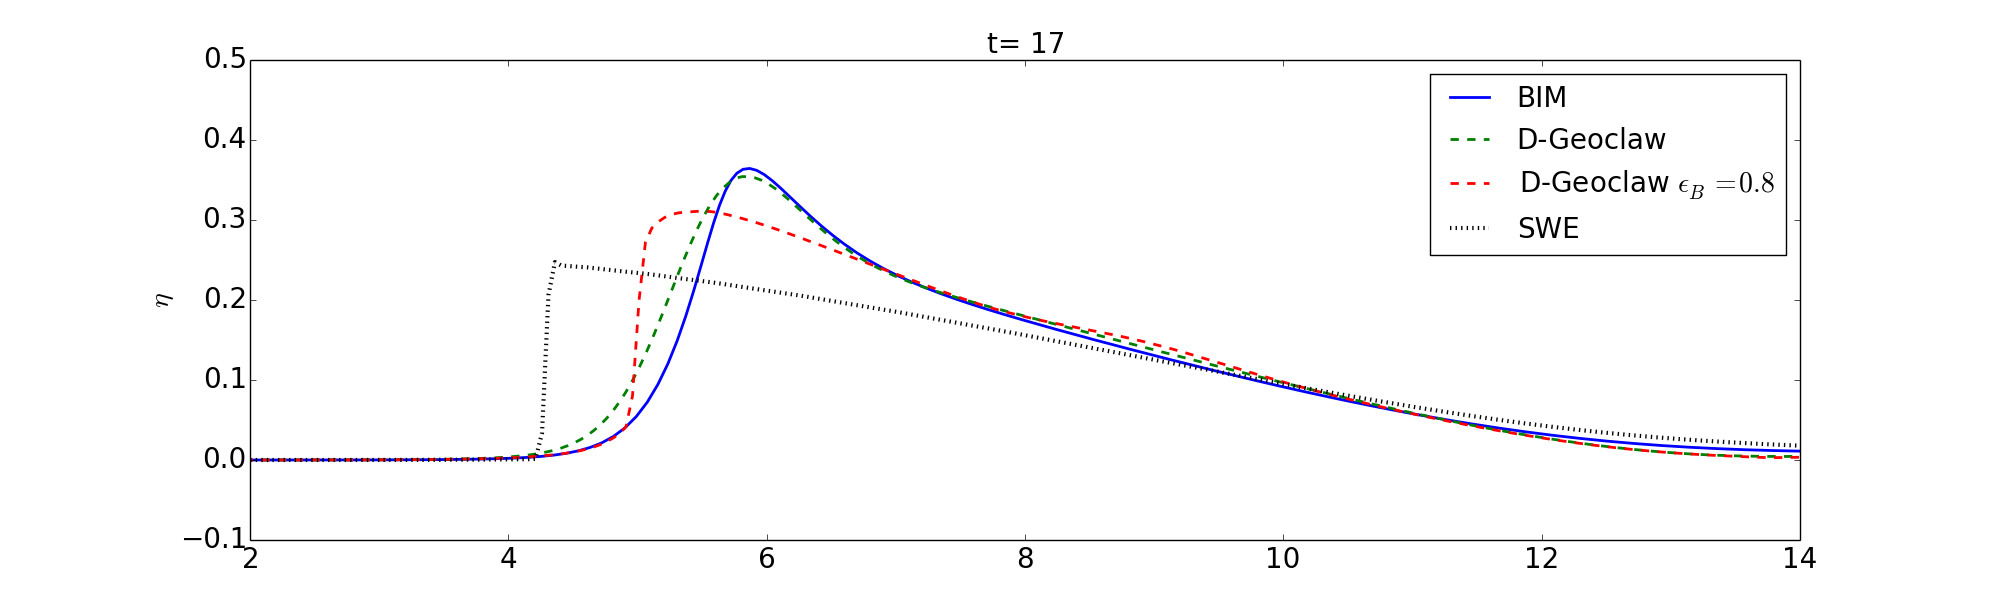
\includegraphics[width=.9\textwidth]{_fig/bim_dgeo_etaB8_170.png}\\
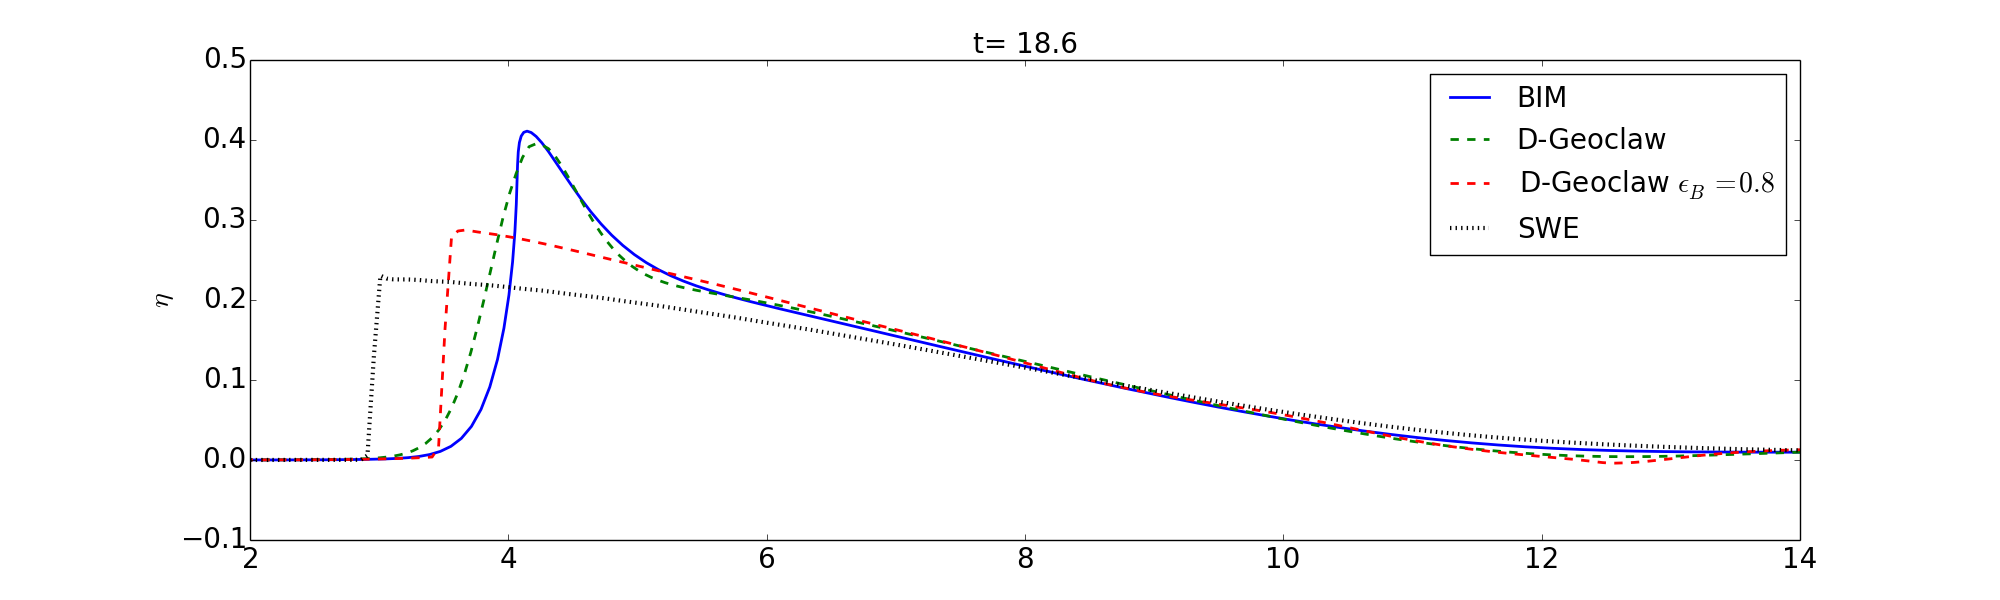
\includegraphics[width=.9\textwidth]{_fig/bim_dgeo_etaB8_186.png}
\caption{Comparison of BIM, \textsc{WaveClaw} and SWE 
with $\epsilon=0.8$ at t =$15$, $17$ and $18.6$.}
\label{fig:dgeo_th08}
\end{figure}

In Figure \ref{fig:dgeo_th08}, snapshots are shown at 
t=$15$, $17$, and $18.6$ from BIM, \textsc{WaveClaw} 
and SWE.
At t=$15$, the difference between BIM and \textsc{WaveClaw}
is small, but the difference becomes noticeable 
in the wave shape and amplitude at t = $17$ and $18.6$ . 
As the governing equations are switched to the shallow water equations,
the wave starts to form a shockfront, and the wave amplitude decreases.

Figure \ref{fig:wave_break_criteria} shows 
the values of the wave breaking criteria at the given crest location. 
With BIM simulations, the wave starts breaking at $x=4.09$ m. 
From \textsc{WaveClaw}, the values at $x=4.09$ m are
$A/h=1.97$, $u_s/c=1.04$ and maximum angle=$39.1^\circ$
where the maximum angle refers to 
the maximum slope of steepening wave.

\begin{figure}[!htb]
\centering
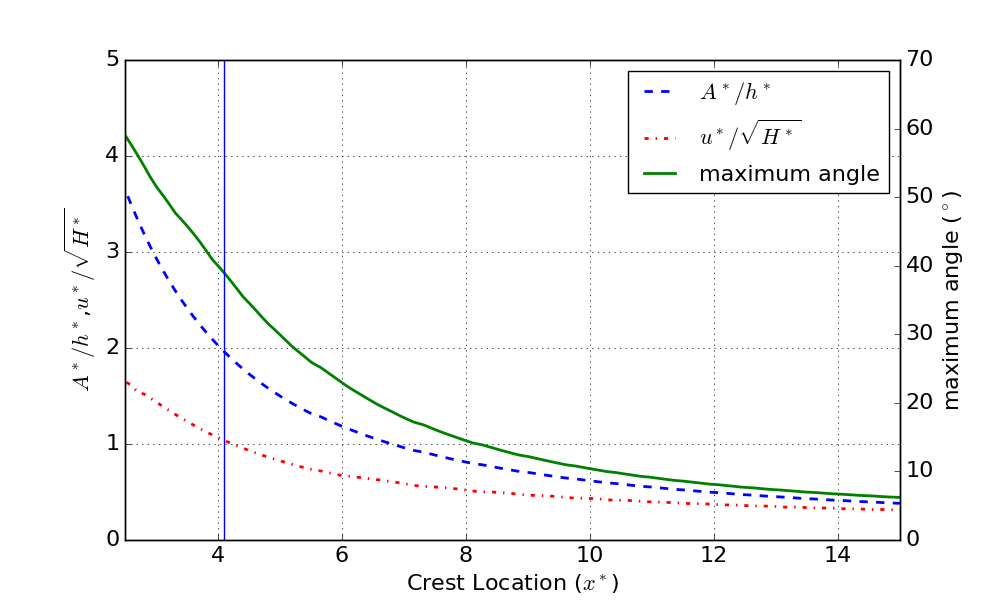
\includegraphics[width=.7\textwidth]{_fig/wave_break}
\caption{Plot of $A/\eta$, $u_s/c$ and maximum angle of waves vs. crest location. 
BIM shows the wave break at $x=4.09$. }
\label{fig:wave_break_criteria}
\end{figure}

\subsection{Wave Energy}

The wave energy is conserved when the wave is smooth, 
and decreases as the wave forms a shock or breaks.
The wave energy expressions 
for the shallow water equations and Boussinesq equations
are $E_0$ and $E_0+E_1$  respectively, 
which are given in (\ref{eq:energy_e0}) and (\ref{eq:energy_e1}). 

In Figure \ref{fig:energy_dgeo_swe}, 
the wave energy $E_0$ and $E_0+E_1$ are shown. 
The energy denotes the aggregate 
of the wave energy in the entire computational domain 
at the given crest location.
On the left figure, 
the energy $E_0$ is well-preserved 
for the shallow water equations 
before the wave forms a shock,
and then the energy dissipates after a shock is formed.
On the right figure, 
$E_0+E_1$ is well-preserved for the \textsc{WaveClaw},
and this value decreases slightly as the wave steepens
near the shoreline.
When the threshold $\epsilon_B=0.8$ is used,
the energy $E_0+E_1$ is well-preserved 
as shown on the right figure before the threshold is reached. 
When the crest is located
at $x=8.03227$ m with $\epsilon_B=0.8$, 
the wave energy $E_0$ on the left figure 
does not decrease immediately.
The energy $E_0$ is preserved for a while, 
then starts to decrease as a shock is formed. 

\begin{figure}[!htb]
    \centering
    \begin{subfigure}[b]{0.45\textwidth}
        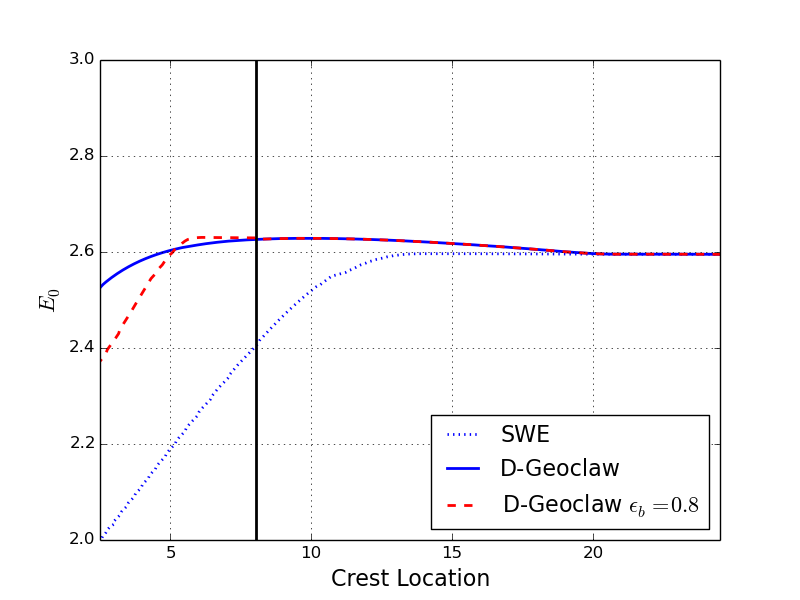
\includegraphics[width=\textwidth]{_fig/e0_dgeo_eb08.png}
        \caption{$E_0$}
        \label{fig:e0_dgeo_eb08}
    \end{subfigure}
    \begin{subfigure}[b]{0.45\textwidth}
        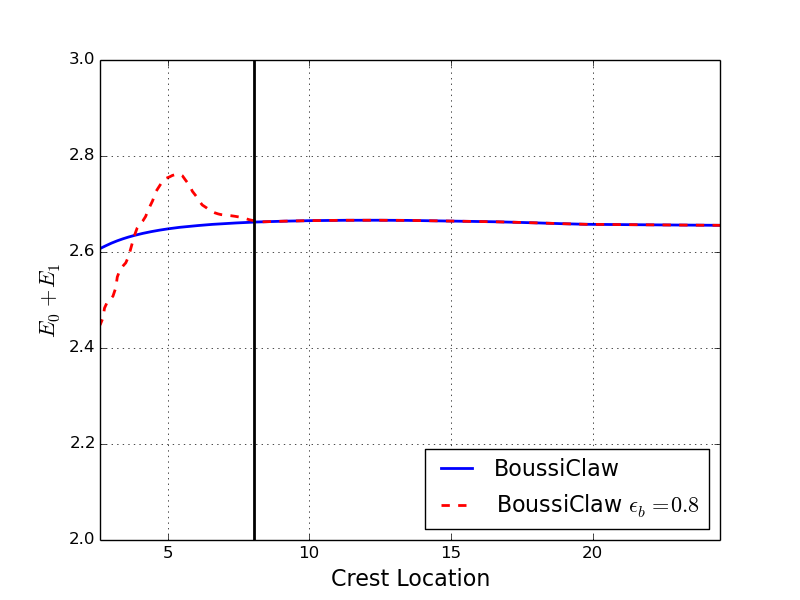
\includegraphics[width=\textwidth]{_fig/e1_dgeo_eb08.png}
        \caption{$E_0+E_1$}
        \label{fig:e1_dgeo_eb08}
    \end{subfigure}
    \caption{Energy plots of SWE and \textsc{WaveClaw}.
    The vertical line is at $x=8.03227$ m where $\epsilon_B=0.8$,
    and the governing equations are switched to the SWE from
    the Boussinesq equations. }
    \label{fig:energy_dgeo_swe}
\end{figure}

\section{Conclusion}
{\em What should the main conclusions be}
\begin{itemize}
\item Dispersive Geoclaw works.
\item Shallow water models and composite Boussinesq/NLSW models
      may give large errors in breaking point and wave shape
\item Breaking does not really occur before the local amplitude is much higher than 0.8 time the depth -- a limit that is inspired by the
existence of solitary wave solution in full potential theory.
The 0.8 limit  may be better on even gentler slopes.
\item Effects of nonlinearities in the dispersion does influence the 
solution markedly, when accumulated up to the point of breaking.
\end{itemize}
%From the laboratory experiments, Titov and Synolakis (1995) \cite{titov1995modeling} determined that the wave breaking starts when the non-dimensional distance from the shoreline is about $x^*=2.5$. The breaking point was determined by approximating the wave front and crest paths. When two paths coincide, it is assumed that the wave starts breaking. 

\section*{References}

\bibliography{mybibfile}

\appendix

\section{Comparison of the Boussinesq equations}
\label{append:a}

A class of the Boussinesq-type equations can be written 
in the following form,
\begin{flalign}
& (H)_t + (Hu)_x = 0, \\
& (Hu)_t + \left( Hu^2 + \frac{gH²}{2} \right)_x + gHh_x + \psi = 0,
\end{flalign}
where $\psi$ represents dispersion terms.
If 
\begin{flalign}
\psi = \frac{Hh^2}{6} u_{xxt} - \frac{Hh}{2} (hu)_{xxt},
\label{eq:peregrine_disp}
\end{flalign}
then these are called 
the Peregrine's equations.

The Boussinesq equations by Sch{\"a}ffer and Madsen \cite{schaffer1995further}
can be approximately reduced to the Peregrine's form when $B=0$.
Since $H=h+\eta$, the Madsen's dispersion term (\ref{eq:madsen_new_disp_x}) can be written as, 
\begin{flalign}
\psi = & \frac{1}{6}h^3 \left(\frac{Hu}{h} \right)_{xxt}
- \frac{1}{2}h^2 (Hu)_{xxt} \nonumber \\
= & \frac{1}{6}h^3 u_{xxt}
+ \frac{1}{6}h^3 \left( \frac{\eta u}{h} \right)_{xxt}
- \frac{1}{2}h^2 (hu)_{xxt} - \frac{1}{2}h^2 (\eta u)_{xxt} \nonumber \\
= & \frac{H h^2}{6} u_{xxt} - \frac{H h}{2} (hu)_{xxt} \nonumber \\
&- \frac{\eta h^2}{6} u_{xxt}
+ \frac{h^3}{6} \left( \frac{\eta u}{h} \right)_{xxt}
+ \frac{\eta h}{2} (hu)_{xxt}
- \frac{h^2}{2} (\eta u)_{xxt} \label{eq:append_schaffer_disp1} \\
= & \frac{H h^2}{6} u_{xxt} - \frac{H h}{2} (hu)_{xxt}
+ \mathcal{O}(\epsilon). \nonumber
\end{flalign}
Because the last four terms in (\ref{eq:append_schaffer_disp1})
are $\mathcal{O}(\epsilon$).
The dispersion terms of Sch{\"a}ffer and Madsen are approximately same as
the Peregrine's. 
Because of the higher order terms in (\ref{eq:append_schaffer_disp1}),
Sch{\"a}ffer and Madsen's wave model has lower peak at the breaking
than Peregrine's model. 

Now use $H=h+\eta$ and $\eta_t = H_t = -(Hu)_x$,
and assume $\eta_{xx}$ is small. Then $\psi$ can be rewritten as
\begin{flalign*}
\psi = & \frac{1}{6}h^3 \left(\frac{Hu}{h} \right)_{xxt}
- \frac{1}{2}h^2 (Hu)_{xxt} \\
= & - Hh h_xu_{xt} -\frac{1}{3} H h^2 u_{xxt}- H h \eta_xu_{xt} \\
& - \frac{1}{6} Hh \eta u_{xxt} 
+ \frac{1}{6} h \eta^2 u_{xxt} + h \eta (h+\eta)_x u_{xt} 
+ \frac{1}{6} h^3 \left( \frac{\eta u}{h} \right)_{xxt}
\end{flalign*}
Meanwhile
\begin{flalign*}
\left( \frac{\eta u}{h} \right)_{xxt} 
= & -\frac{2 h_x}{h^2}\eta u_{xt} 
+ \frac{2}{h} \eta_x u_{xt}
+ \frac{1}{h} \eta u_{xxt} 
+ \frac{2 h_x}{h^2} (Hu)_x u_{x} \\
&- \frac{2}{h} (Hu)_{xx} u_x 
- \frac{1}{h} (Hu)_x u_{xx}.
\end{flalign*}

Therefore $\psi$ reduces to 
\begin{flalign*}
\psi 
= & Hh\eta_xu_{xt} + \left( \frac{2}{3} h_x \eta  
- \frac{2}{3} h \eta_x  \right) hu_{xt} \\
& + \frac{1}{6} h^3 \left(\frac{2 h_x}{h^2} (Hu)_x u_{x}
- \frac{2}{h} (Hu)_{xx} u_x 
- \frac{1}{h} (Hu)_x u_{xx}  \right)  \\
= & - Hh h_xu_{xt} -\frac{1}{3} H h^2 u_{xxt}
+ \left( \frac{2}{3} h_x \eta  
- \frac{2}{3} h \eta_x  \right) hu_{xt} \\
& + \frac{1}{6} h^3 \left(\frac{2 h_x}{h^2} (Hu)_x u_{x}
- \frac{2}{h} (Hu)_{xx} u_x 
- \frac{1}{h} (Hu)_x u_{xx}  \right) \\
\end{flalign*}
Now consider the last term 
\begin{flalign*}
 & \frac{1}{6} h^3 \left(\frac{2 h_x}{h^2} (Hu)_x u_{x}
- \frac{2}{h} (Hu)_{xx} u_x 
- \frac{1}{h} (Hu)_x u_{xx}  \right) \\
= & \frac{1}{3} h \left( h_x (Hu)_x u_{x}
- h (Hu)_{xx} u_x 
- \frac{h}{2} (Hu)_x u_{xx}  \right) \\
= & \frac{1}{3} h \left( h_x \left( H_xu + Hu_x \right) u_{x}
- h \left( 2H_xu_x + Hu_{xx} \right) u_x 
- \frac{h}{2} (H_xu + Hu_x) u_{xx}  \right) \\
= & \frac{1}{3} h \left( h_x H (u_x)^2 
- 2H_x h (u_x)^2 - H h u_x u_{xx} 
- \frac{h}{2} H_x u u_{xx} - \frac{h}{2} H u_x u_{xx} \right) \\
= & \frac{1}{3} h \left( \left( h_x H - 2H_x h \right) (u_x)^2 
- \frac{3 H h}{2} u_x u_{xx} 
- \frac{h}{2} H_x u u_{xx} \right) \\
\end{flalign*}


If we rearrange (\ref{eq:madsen_new_disp_x}) and
assume that $h_x\eta$, $h_{xx}$ and $\eta_{xx}$ are small,
then 
the Madsen's dispersion terms can be written as
\begin{flalign*}
\psi 
\approx & - Hh h_xu_{xt} -\frac{Hh^2}{3} u_{xxt}- H h \eta_xu_{xt}
- \frac{1}{6} Hh \eta u_{xxt} 
+ \frac{1}{6} h^3 \left( \frac{\eta u}{h} \right)_{xxt}.
\end{flalign*}
Since $\eta_t = -(Hu)_x$, we have
\begin{flalign*}
\left( \frac{\eta u}{h} \right)_{xxt} 
\approx & \frac{2 \eta_x}{h} u_{xt}
+ \frac{\eta}{h} u_{xxt}  &+ \frac{2 h_x}{h^2} (Hu)_x u_{x}
- \frac{2}{h} (Hu)_{xx} u_x 
- \frac{1}{h} (Hu)_x u_{xx}.
\end{flalign*}
Plugging in and dropping small terms yields to 
\begin{flalign}
\psi 
\approx & - Hh h_xu_{xt} -\frac{Hh^2}{3} u_{xxt}- H h \eta_xu_{xt} 
- \frac{1}{6} Hh \eta u_{xxt} \nonumber \\
& +\frac{h^2\eta_x}{3} u_{xt}
+ \frac{h^2\eta}{6} u_{xxt} + \frac{h h_x}{3} (Hu)_x u_{x}
- \frac{h^2}{3} (Hu)_{xx} u_x 
- \frac{h^2}{6} (Hu)_x u_{xx} \nonumber \\
\approx & - Hh h_xu_{xt} -\frac{Hh^2}{3} u_{xxt}- H h \eta_xu_{xt} \nonumber \\
& +\frac{h^2\eta_x}{3} u_{xt}
 + \frac{h h_x}{3} (Hu)_x u_{x}
- \frac{h^2}{3} (Hu)_{xx} u_x 
- \frac{h^2}{6} (Hu)_x u_{xx}. \label{eq:madsen_disp_v3}
\end{flalign}
%\marginpar{\small I am not sure how to conclude the relation between Boussinesq and Serre.}

The Serre's equations of Su and Gardner \citep{su1969korteweg}
has the following dispersion terms,
\begin{flalign}
\psi= &-Hhh_xu_{xt} - \frac{Hh^2}{3}u_{xxt}
- Hh\eta_xu_{xt} \nonumber \\
& - \frac{2}{3} Hh\eta u_{xxt}
+ \frac{Hh^2}{3}\left[ (u_x)^2-uu_{xx} \right]_x.
\label{eq:serre_disp}
\end{flalign}
It is observed that (\ref{eq:madsen_disp_v3}) and (\ref{eq:serre_disp}) share common terms.
Numerical results also show that Sch{\"a}ffer and Madsen's 
model is more similar to Serre's equations than Peregrine's equations.

\section{Stability of the hybrid scheme}
\label{append:stab}

In order to investigate the stability of the proposed hybrid numerical scheme,
we consider a linearized Benjamin-Bona-Mahony (BBM)
equation (Benjamin et al., 1972 \cite{benjamin1972model}),
which is a class of the Boussinesq-type equations. 
The PDE is given as follows,
\begin{align}
u_t + u_x = u_{txx}.
\label{eq:basic_1}
\end{align}
In order to apply the hybrid scheme,
the equation (\ref{eq:basic_1}) is rearranged as
\begin{align}
(I-D^2)(u_t + u_x) +D^2u_x = 0, \label{eq:basic_2}
\end{align}
where $D=\partial_x$.
Then we are required to solve the following PDE,
\begin{align}
\left\{
\begin{array}{l}
u_t + u_x + S = 0, \\
\left(I-D^2 \right)S = D^3 u .
\end{array}
\right.
\end{align}
When the hybrid scheme is applied, the advection equation
\begin{align}
u_t + u_x = 0,
\label{eq:append_advec}
\end{align}
is solved with the finite volume method, 
and then the fractional step method is applied to
the following equation,
\begin{align*}
u_t + S = 0.
\end{align*}

If we use the centered difference approximation of $O(\Delta x^2)$
accuracy, and the four-stage Runge-Kutta scheme for time stepping,
then we have,
\begin{align*}
U_1 &:= u^n \\
U_2 &:= u^n - \frac{\Delta t}{2}S_1, \quad  \textrm{where}\quad 
(I-D^2)S_1 = D^3 U_1, \\
U_3 &:= u^n - \frac{\Delta t}{2}S_2, \quad  \textrm{where}\quad
(I-D^2)S_2 = D^3 U_2, \\
U_4 &:= u^n - \Delta tS_3, \quad  \textrm{where}\quad
(I-D^2)S_3 = D^3 U_3, \\
u^{n+1} & = u^n -\frac{\Delta t}{6} \left[
S_1 + 2S_2 + 2S_3 + S_4
\right],  \quad  \textrm{where}\quad
(I-D^2)S_4 = D^3 U_4.
\end{align*}
For each step, $S_i$'s are computed from
\begin{align*}
& (S_i)_j - \frac{(S_i)_{j+1}-2(S_i)_j+(S_i)_{j-1}}{\Delta x^2} = 
\frac{u_{j+2} - 2u_{j+1} +2u_{j-1} -u_{j-2}}{2\Delta x^3}.
\end{align*}
In order to investigate the stability with von Neumann analysis,
replace $u_j= e^{i\xi j \Delta x}$ and  $(S_1)_j= \beta e^{i\xi j \Delta x}$. 
Simplification gives
\begin{align*}
&\beta \left( 1 - \frac{-2+2\cos(\xi \Delta x) }{\Delta x^2} \right) = 
\frac{\sin(2\xi \Delta x) - 2 \sin(\xi \Delta x)}{\Delta x^3} i, \\
& \beta = \frac{ -2\sin(\xi \Delta x)(1-  \cos(\xi \Delta x)) }
                     { \Delta x^3 +2\Delta x(1-\cos(\xi \Delta x))} i.
\end{align*}
Note that $\beta$ is a purely imaginary number.
If we replace the four-stage Runge-Kutta scheme with
$u_j= e^{i\xi j \Delta x}$ and  $(S_1)_j= \beta e^{i\xi j \Delta x}$, then we have
\begin{align*}
&S_1 = \beta e^{i\xi j \Delta x} ,
 \quad U_2 = \left(1-\frac{\Delta t\beta}{2} \right) e^{i\xi j \Delta x}\\
&S_2 = \beta \left(1-\frac{\Delta t\beta}{2} \right) e^{i\xi j \Delta x} ,
 \quad U_3 = \left(1- \frac{\Delta t\beta}{2}+\frac{(\Delta t\beta)^2}{4} \right) e^{i\xi j \Delta x}\\
&S_3 =  \beta\left(1- \frac{\Delta t\beta}{2}+\frac{(\Delta t\beta)^2}{4} \right)  e^{i\xi j \Delta x} , \\
& U_4 = \left(1-\Delta t\beta
+ \frac{(\Delta t\beta)^2}{2}-\frac{(\Delta t\beta)^3}{4} \right) e^{i\xi j \Delta x},\\
&S_4 = \beta \left(1-\Delta t\beta
+ \frac{(\Delta t\beta)^2}{2}-\frac{(\Delta t\beta)^3}{4} \right) e^{i\xi j \Delta x}.
\end{align*}
Thus the growth factor $g(\xi)$ is
\begin{align*}
g(\xi)= & 1-\frac{\Delta t}{6}\bigg[ \beta + 
2 \beta \left(1-\frac{\Delta t\beta}{2} \right) +
2 \beta\left(1- \frac{\Delta t\beta}{2}+\frac{(\Delta t\beta)^2}{4} \right) \\ 
&+ \beta \left(1-\Delta t\beta
+ \frac{(\Delta t\beta)^2}{2}-\frac{(\Delta t\beta)^3}{4} \right)
\bigg] \\
= & 1-\frac{1}{6}\left(
6\Delta t\beta -3(\Delta t\beta)^2 +(\Delta t\beta)^3-\frac{(\Delta t\beta)^4}{4}
\right).
\end{align*}
Since $\beta$ is an imaginary number,
let $\Delta t\beta= \gamma i$ for some real $\gamma$, and then we have
\begin{align*}
g(\gamma) & = 1-
\frac{1}{2}\gamma^2 +\frac{\gamma^4}{24} + \left(\frac{\gamma^3}{6} -\gamma \right)i \\
|g(\gamma)|^2 & = 1 + \frac{1}{4}\gamma^4 + \frac{\gamma^8}{24^2} -\gamma^2 + \frac{\gamma^4}{12}
-\frac{\gamma^6}{24} + \gamma^2 + \frac{\gamma^6}{36} -\frac{\gamma^4}{3} \\
& = 1 -\frac{1}{72}\gamma^6 + \frac{1}{576}\gamma^8.
\end{align*}
If $|\gamma|<2\sqrt{2}$, then $|g(\gamma)|<1$. 
The sufficient condition for stability is 
\begin{align}
\left| \frac{\Delta t}{\Delta x} \cdot \frac{ \sin(\xi \Delta x)(1-  \cos(\xi \Delta x)) }
                     { \Delta x^2 +2(1-\cos(\xi \Delta x))} \right| < \sqrt{2}, 
                     \quad \textrm{for~} \forall \xi \Delta x.
\end{align}
For small $\Delta x$, this condition approximately reduces to
\[
\frac{\Delta t}{\Delta x} < 2\sqrt{2}.
\]
The CFL condition for the advection equation
(\ref{eq:append_advec}) is a sufficient condition. 
Therefore, if the CFL condition is satisfied in the advection equation,
the fractional step is always stable with the suggested numerical scheme. 

\section{Energy estimates and dissipation}
\label{append:energy}

\subsection{Velocity field}

To derive the energy estimates for the Boussinesq-type equations, 
we define the depth-averaged velocity as,  
\begin{flalign*}
\bar{u} = \frac{1}{H}\int_{-h}^{\epsilon \eta} u dz .
\end{flalign*}
Then the velocity $u$ can be expressed as
$u = \bar{u} + \mu^2 u_1$ where
\begin{align}
\int_{-h}^{\epsilon \eta} u_1 dz=0. \label{eq:avg_u1}
\end{align}
Then the kinematic boundary condition at the bottom and zero divergence
implies
\begin{flalign*}
w = -h_x u  - \bar{u}_x (z+h) + O(\mu^2). 
\end{flalign*}

\subsection{Energy integrals}

The potential energy density per horizontal area is 
\begin{flalign*}
V = \int_{-h}^{\epsilon \eta} g z dz = \frac{1}{2}\epsilon^2 g \eta^2 
- \frac{1}{2} g h^2, 
\end{flalign*}
where the last term $\frac{1}{2} g h^2$ is the equilibrium energy.
The kinematic energy density has two contributions,
\begin{flalign*}
T=T_u+T_w; 
\quad T_u = \frac{1}{2}\epsilon^2 \int_{-h}^{\epsilon \eta} u^2 dz, 
\quad T_w = \frac{1}{2}\epsilon^2 \mu^2 \int_{-h}^{\epsilon \eta} w^2 dz. 
\end{flalign*}
For the horizontal part, $T_u$ is 
\begin{flalign*}
T_u = \frac{1}{2}\epsilon^2 \int_{-h}^{\epsilon \eta} u^2 dz
= \frac{1}{2}\epsilon^2 \int_{-h}^{\epsilon \eta} 
\bar{u}^2+2\mu^2\bar{u}u_2 + \mu^4u_1^2 dz
= \frac{1}{2}\epsilon^2 H \bar{u}^2 + O(\epsilon^2 \mu^4),
\end{flalign*}
since $\bar{u}$ is independent of $z$ and by (\ref{eq:avg_u1}).
Assuming $\frac{1}{H}\int_{-h}^{\epsilon \eta} u^2 dz = \bar{u}^2$,
the vertical part is 
\begin{flalign*}
\quad T_u & = \frac{1}{2}\epsilon^2 \mu^2 \int_{-h}^{\epsilon \eta} 
h_x^2u^2 +2h_xu\bar{u}_x(z+h)
+ \bar{u}_x^2 (z+h)^2 dz + O(\epsilon^2\mu^4) \\
& = \frac{1}{2}\epsilon^2 \mu^2 H
\left(
h_x^2 \bar{u}^2 + H h_x\bar{u} \bar{u}_x + \frac{1}{3} H^2 \bar{u}_x^2
\right) + O(\epsilon^2\mu^4).
\end{flalign*}
Thus the energy of a wave can be approximated as 
\begin{flalign*}
& E = \epsilon^2 \left( E_0 +\mu^2 E_1 + O (\mu^4)\right)
\end{flalign*}
where
\begin{flalign*}
& E_0 = \frac{1}{2}\left( g\eta^2 + H\bar{u}^2 \right), \\
& E_1 = \frac{1}{6}H^3\bar{u}_x^2
+ \frac{1}{2}H^2h_x\bar{u}\bar{u}_x + \frac{1}{2}Hh_x^2\bar{u}^2.
\end{flalign*}

\end{document}
---
